%% LyX 2.3.4.2 created this file.  For more info, see http://www.lyx.org/.
%% Do not edit unless you really know what you are doing.
\documentclass[english,dvipsnames,aspectratio=169]{beamer}
\usepackage{mathptmx}
\usepackage{eulervm}
\usepackage[T1]{fontenc}
\usepackage[latin9]{inputenc}
\usepackage{babel}
\usepackage{amstext}
\usepackage{amssymb}
\usepackage{graphicx}
\usepackage{ifthen}
\usepackage{xcolor}
\usepackage{xspace}
\usepackage{tikz}
\usetikzlibrary{tikzmark}
\usetikzlibrary{calc}
\usepackage{pgfplots}
%\pgfplotsset{compat=1.17}
\usepackage{booktabs}
\usepackage{xpatch}

\xpatchcmd{\itemize}
  {\def\makelabel}
  {\ifnum\@itemdepth=1\relax
     \setlength\itemsep{2ex}% separation for first level
   \else
     \ifnum\@itemdepth=2\relax
       \setlength\itemsep{1ex}% separation for second level
     \else
       \ifnum\@itemdepth=3\relax
         \setlength\itemsep{0.5ex}% separation for third level
   \fi\fi\fi\def\makelabel
  }
 {}
 {}

\ifx\hypersetup\undefined
  \AtBeginDocument{%
    \hypersetup{unicode=true,pdfusetitle,
 bookmarks=true,bookmarksnumbered=false,bookmarksopen=false,
 breaklinks=false,pdfborder={0 0 0},pdfborderstyle={},backref=false,colorlinks=true,
 allcolors=NYUPurple,urlcolor=LightPurple}
  }
\else
  \hypersetup{unicode=true,pdfusetitle,
 bookmarks=true,bookmarksnumbered=false,bookmarksopen=false,
 breaklinks=false,pdfborder={0 0 0},pdfborderstyle={},backref=false,colorlinks=true,
 allcolors=NYUPurple,urlcolor=LightPurple}
\fi

\makeatletter

%%%%%%%%%%%%%%%%%%%%%%%%%%%%%% LyX specific LaTeX commands.
%% Because html converters don't know tabularnewline
\providecommand{\tabularnewline}{\\}

%%%%%%%%%%%%%%%%%%%%%%%%%%%%%% Textclass specific LaTeX commands.
% this default might be overridden by plain title style
\newcommand\makebeamertitle{\frame{\maketitle}}%
% (ERT) argument for the TOC
\AtBeginDocument{%
  \let\origtableofcontents=\tableofcontents
  \def\tableofcontents{\@ifnextchar[{\origtableofcontents}{\gobbletableofcontents}}
  \def\gobbletableofcontents#1{\origtableofcontents}
}

%%%%%%%%%%%%%%%%%%%%%%%%%%%%%% User specified LaTeX commands.
\usetheme{CambridgeUS} 
\beamertemplatenavigationsymbolsempty


% Set Color ==============================
\definecolor{NYUPurple}{RGB}{87,6,140}
\definecolor{LightPurple}{RGB}{165,11,255}


\setbeamercolor{title}{fg=NYUPurple}
\setbeamercolor{frametitle}{fg=NYUPurple}

\setbeamercolor{background canvas}{fg=NYUPurple, bg=white}
\setbeamercolor{background}{fg=black, bg=NYUPurple}

\setbeamercolor{palette primary}{fg=black, bg=gray!30!white}
\setbeamercolor{palette secondary}{fg=black, bg=gray!20!white}
\setbeamercolor{palette tertiary}{fg=gray!20!white, bg=NYUPurple}

\setbeamertemplate{headline}{}
\setbeamerfont{itemize/enumerate body}{}
\setbeamerfont{itemize/enumerate subbody}{size=\normalsize}
\setbeamerfont{itemize/enumerate subsubbody}{size=\normalsize}

\setbeamercolor{parttitle}{fg=NYUPurple}
\setbeamercolor{sectiontitle}{fg=NYUPurple}
\setbeamercolor{sectionname}{fg=NYUPurple}
\setbeamercolor{section page}{fg=NYUPurple}
%\setbeamercolor{description item}{fg=NYUPurple}
%\setbeamercolor{block title}{fg=NYUPurple}

\setbeamertemplate{blocks}[rounded][shadow=false]
\setbeamercolor{block body}{bg=normal text.bg!90!NYUPurple}
\setbeamercolor{block title}{bg=NYUPurple!30, fg=NYUPurple}



\AtBeginSection[]{
  \begin{frame}
  \vfill
  \centering
\setbeamercolor{section title}{fg=NYUPurple}
 \begin{beamercolorbox}[sep=8pt,center,shadow=true,rounded=true]{title}
    \usebeamerfont{title}\usebeamercolor[fg]{title}\insertsectionhead\par%
  \end{beamercolorbox}
  \vfill
  \end{frame}
}

\makeatother

\setlength{\parskip}{\medskipamount} 

\input ../macros

\begin{document}
\input ../rosenberg-macros

\title[DS-GA 1003]{SVM}
\author{He He\\\vspace{2em}{
    Slides based on Lecture
    \href{https://davidrosenberg.github.io/mlcourse/Archive/2019/Labs/3-SVM-Slides.pdf}{Lab 3}
    from David Rosenberg's \href{https://github.com/davidrosenberg/mlcourse}{course material}.
}}

\date{Feb 15, 2022}
\institute{CDS, NYU}

\makebeamertitle
\mode<article>{Just in article version}

\begin{frame}
    Today's lecture: 
    \begin{itemize}
        \item Support Vector Machines: one of the most widely used classification model
        \item We will focus on linear SVM today (non-linear SVM next week!)
        \item Plan:
            \begin{itemize}
                \item Derive the SVM learning objective (in two ways)
                \item Solve the optimization problem 
                \item Get insight from its dual problem
            \end{itemize}
        \item (Requires some background knowledge on convex optimization)
    \end{itemize}
\end{frame}

\begin{frame}{Part I: Derive the SVM Objective}
    \begin{itemize}
        \item Start with the inductive bias: what makes a good linear decision boundary?
        \item Start with the loss function and regularization
    \end{itemize}
\end{frame}

\section{Maximum Margin Classifier}

\begin{frame}
    {Linearly Separable Data}
    Consider a linearly separable dataset $\sD$:
    \begin{figure}
        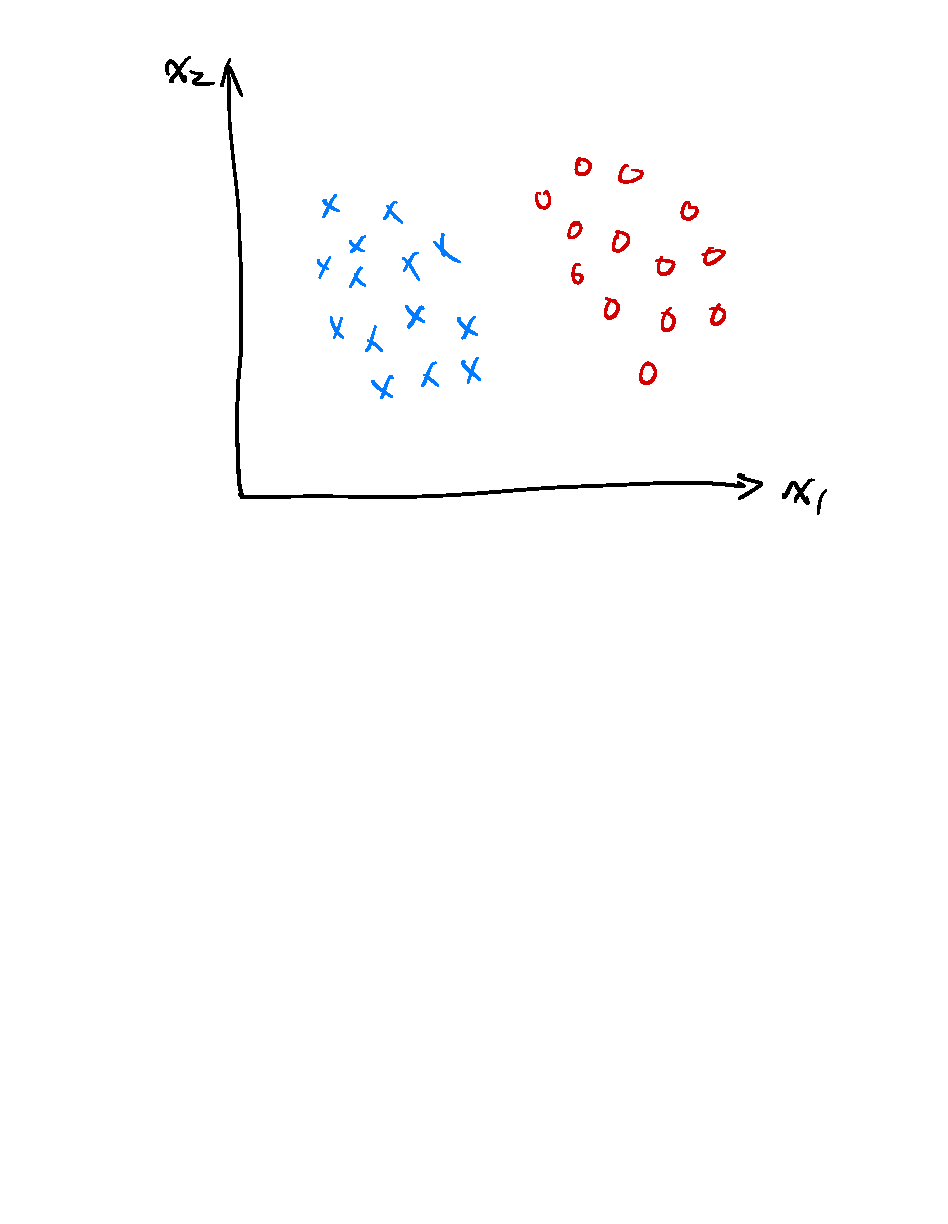
\includegraphics[height=0.5\textheight]{figures/lin-sep-data}
    \end{figure}
    Find a separating hyperplane such that
    \begin{itemize}
        \item $w^Tx_i > 0$ for all $x_i$ where $y_i=+1$
        \item $w^Tx_i < 0$ for all $x_i$ where $y_i=-1$
    \end{itemize}
\end{frame}

\begin{frame}
    {The Perceptron Algorithm}
    \begin{itemize}
        \setlength\itemsep{1ex}
        \item Initialize $w \leftarrow 0$
        \item While not converged (exists misclassified examples)
            \begin{itemize}
                \item For $(x_i, y_i)\in\sD$
                    \begin{itemize}
                        \item If $y_i w^Tx_i < 0$ (wrong prediction)
                        \item Update $w \leftarrow w + y_ix_i$
                    \end{itemize}
            \end{itemize}
    \end{itemize}
    \begin{itemize}
        \item Intuition: move towards misclassified positive examples and away from negative examples
        \item Guarantees to find a zero-error classifier (if one exists) in finite steps
        \item What is the loss function if we consider this as a SGD algorithm?
    \end{itemize}
\end{frame}

\begin{frame}
    {Maximum-Margin Separating Hyperplane}
    For separable data, there are infinitely many zero-error classifiers.

    Which one do we pick?
    \begin{figure}
        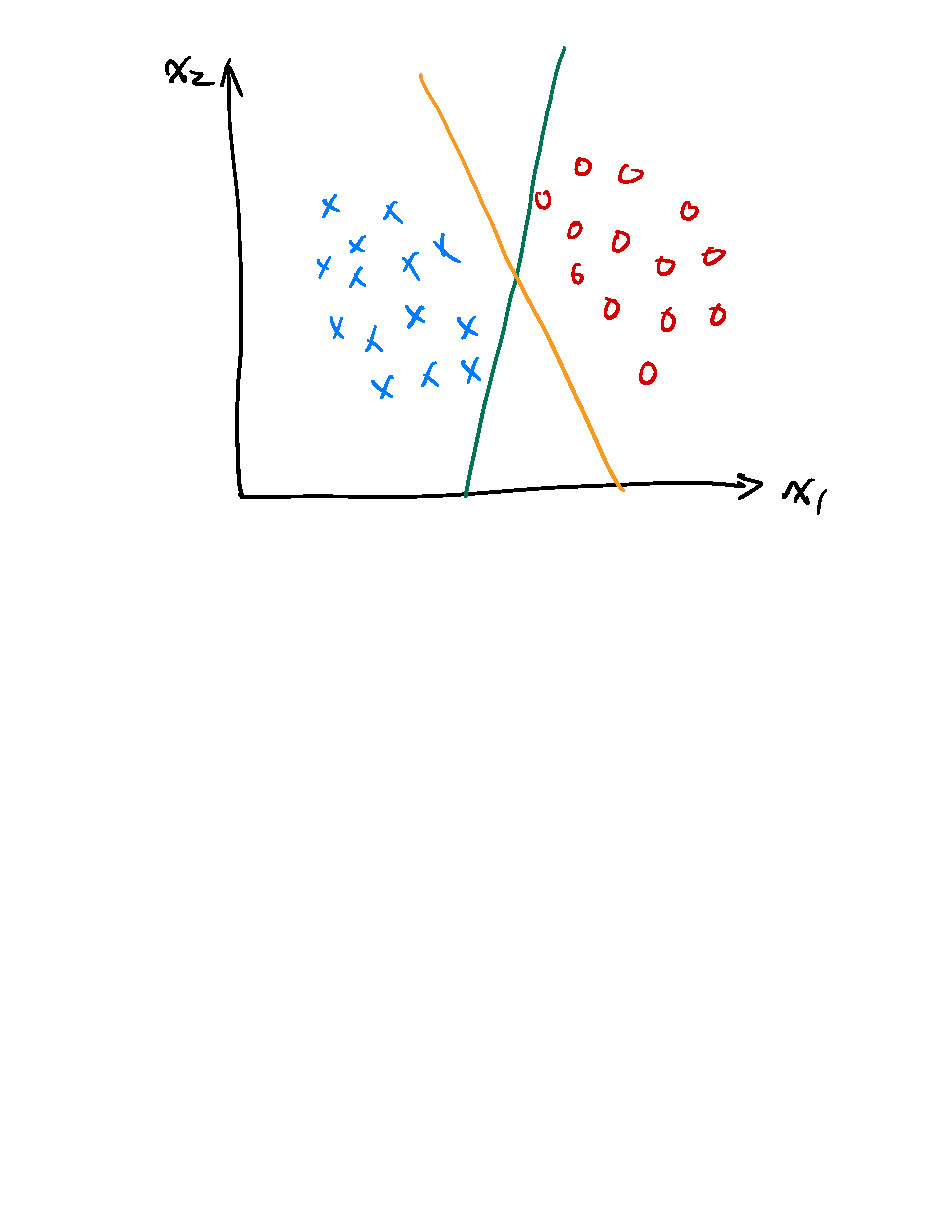
\includegraphics[height=0.5\textheight]{figures/perceptron-hyperplane}
    \end{figure}

    (Perceptron does not return a unique solution.)
\end{frame}

\begin{frame}
    {Maximum-Margin Separating Hyperplane}
    We prefer the classifier that is farthest from both classes of points
    \begin{figure}
        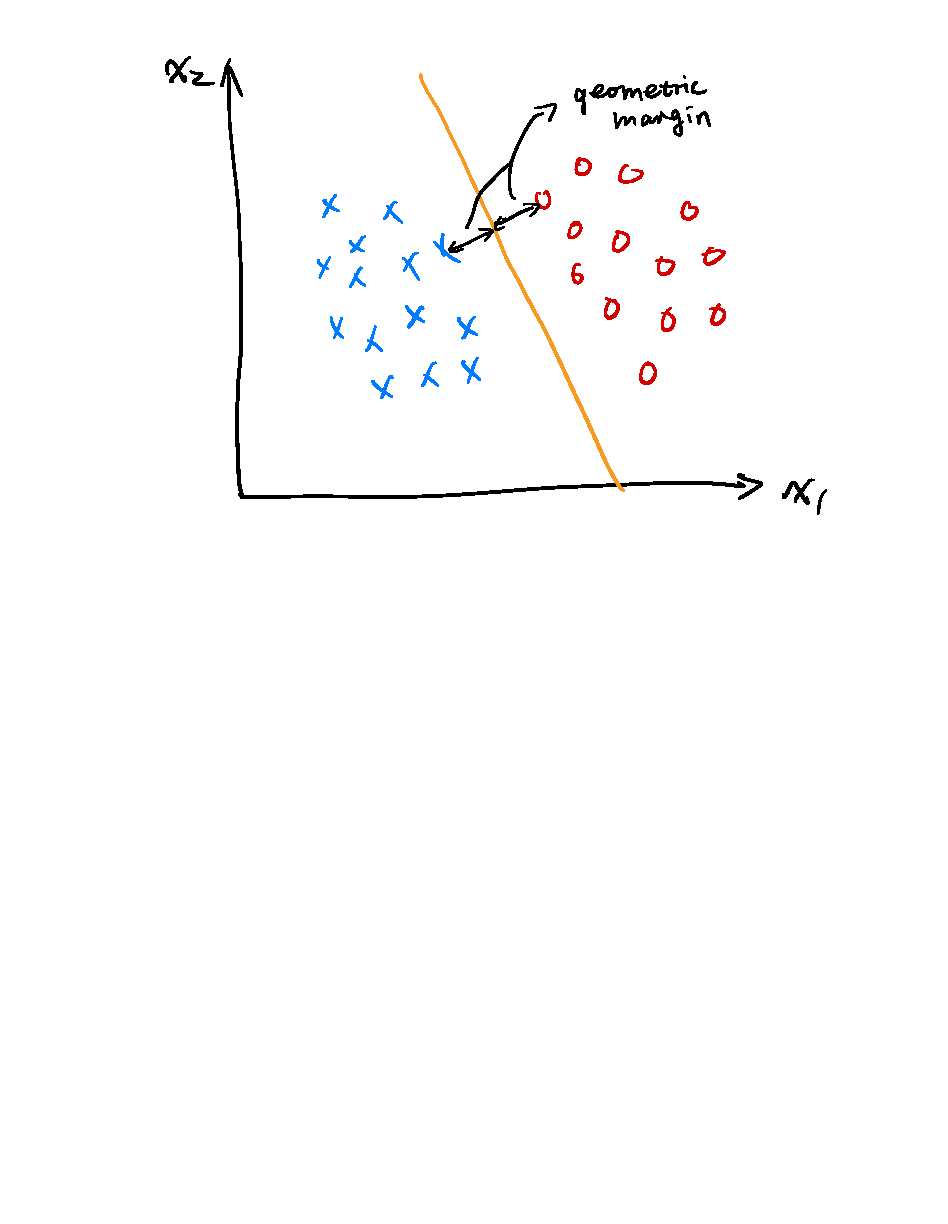
\includegraphics[height=0.5\textheight]{figures/margin}
    \end{figure}
    \begin{itemize}
        \item Geometric margin: smallest distance between the hyperplane and the points 
        \item Maximum margin: \emph{largest} distance to the closest points
    \end{itemize}
\end{frame}

\begin{frame}
    {Geometric Margin}
    We want to maximize the distance between the \hl{separating hyperplane} and the \hl{cloest} points.

    Let's formalize the problem.
    \begin{definition}[separating hyperplane]
    We say $(x_i,y_i)$ for $i=1,\ldots,n$ are \textbf{linearly separable} if there
    is a $w\in\BR^d$ and $b\in\BR$ such that $y_i(w^Tx_i+b)>0$ for all
    $i$. The set $\{v\in\BR^d\mid w^Tv+b=0\}$ is called a \textbf{separating hyperplane}.    
  \end{definition}

    \begin{definition}[geometric margin]
        Let $H$ be a hyperplane that separates the data $(x_i,y_i)$ for $i = 1,\ldots,n$. The \textbf{geometric margin} of this hyperplane is
        $$
        \min_i d(x_i, H),
        $$
    the distance from the hyperplane to the closest data point.
    \end{definition}
\end{frame}

\begin{frame}
    {Distance between a Point and a Hyperplane}
    \vspace{10em}
    \begin{itemize}
        \item Projection of $v\in\BR^d$ onto $w\in\BR^d$:
            $\frac{v\cdot w}{\|w\|_2}$
        \item Distance between $x_i$ and $H$:
            $$
            d(x_i, H) = \left |\frac{w^Tx_i + b}{\|w\|_2}\right |
            = \frac{y_i(w^Tx_i + b)}{\|w\|_2}
            $$
    \end{itemize}
\end{frame}

\begin{frame}
    {Maximize the Margin}
    We want to maximize the geometric margin:
    $$
    \text{maximize} \; \min_{i} d(x_i, H) .
    $$
    Given separating hyperplane $H=\pc{v\mid w^Tv + b = 0}$, we have
    $$
    \text{maximize} \; \min_{i} \frac{y_i(w^Tx_i + b)}{\|w\|_2} .
    $$
    Let's remove the inner minimization problem by
      $$\begin{array}{ll}
      \text{maximize} & M\\
          \text{subject to} & \frac{y_i(w^Tx_i+b)}{\|w\|_2} \geq M \quad\text{for all
        $i$}
    \end{array}$$
    Note that the solution is not unique (why?).
\end{frame}

\begin{frame}
    {Maximize the Margin}
    Let's fix the norm $\|w\|_2$ to $1/M$ to obtain:
      $$\begin{array}{ll}
          \text{maximize} & \frac{1}{\|w\|_2}\\
      \text{subject to} & y_i(w^Tx_i+b) \geq 1 \quad\text{for all
        $i$}
    \end{array}$$
    It's equivalent to solving the minimization problem
      $$\begin{array}{ll}
          \text{minimize} & {\frac{1}{2}\|w\|_2^2}\\
      \text{subject to} & y_i(w^Tx_i+b) \geq 1 \quad\text{for all
        $i$}
    \end{array}$$

    Note that $y_i(w^Tx_i+b)$ is the (functional) margin.

    In words, it finds the minimum norm solution which has a margin of at least 1 on all examples.
\end{frame}

\begin{frame}
    {Soft Margin SVM}
    What if the data is \textit{not} linearly separable?

    For any $w$, there will be points with a negative margin.

    Introduce \textbf{slack variables} to penalize small margin:
      $$\begin{array}{ll}
          \text{minimize} & {\frac{1}{2}\|w\|_2^2}
           + \frac{C}{n}\sum_{i=1}^n \xi_i \\
      \text{subject to} & y_i(w^Tx_i+b) \geq 1 - \xi_i \quad\text{for all
        $i$}\\
          & \xi_i \geq 0 \quad\text{for all $i$}
    \end{array}$$
    \begin{itemize}
        \setlength\itemsep{1ex}
        \item If $\xi_i = 0 \;\forall i$, it's reduced to hard SVM.
        \item What does $\xi_i > 0$ mean?
        \item What does $C$ control?
    \end{itemize}
\end{frame}

\begin{frame}
    {Slack Variables}
    $d(x_i, H) = \frac{y_i(w^Tx_i+b)}{\|w\|_2} \ge \frac{1-\xi_i}{\|w\|_2}$,
    thus $\xi_i$ measures the violation by multiples of the geometric margin:
    \begin{itemize}
        \setlength\itemsep{1ex}
        \item $\xi_i=1$: $x_i$ lies on the hyperplane
        \item $\xi_i=3$: $x_i$ is past 2 margin width beyond the decision hyperplane 
    \end{itemize}
    \begin{figure}
        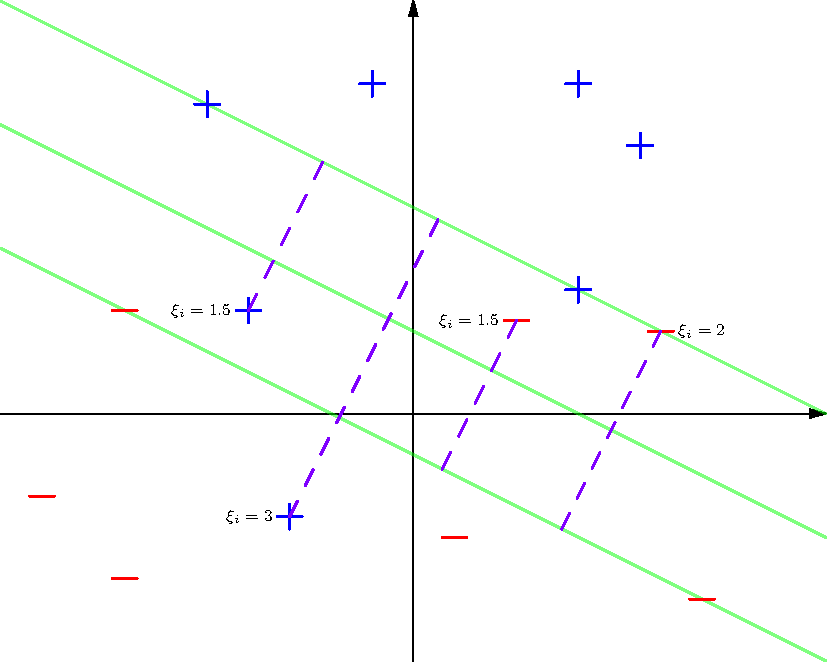
\includegraphics[height=0.6\textheight]{figures/SoftMargin}
    \end{figure}
\end{frame}

\section{Minimize the Hinge Loss}
\begin{frame}
    {Perceptron Loss}
    $$
    \ell(x,y,w) = \max(0, -yw^Tx)
    $$
    \begin{figure}
        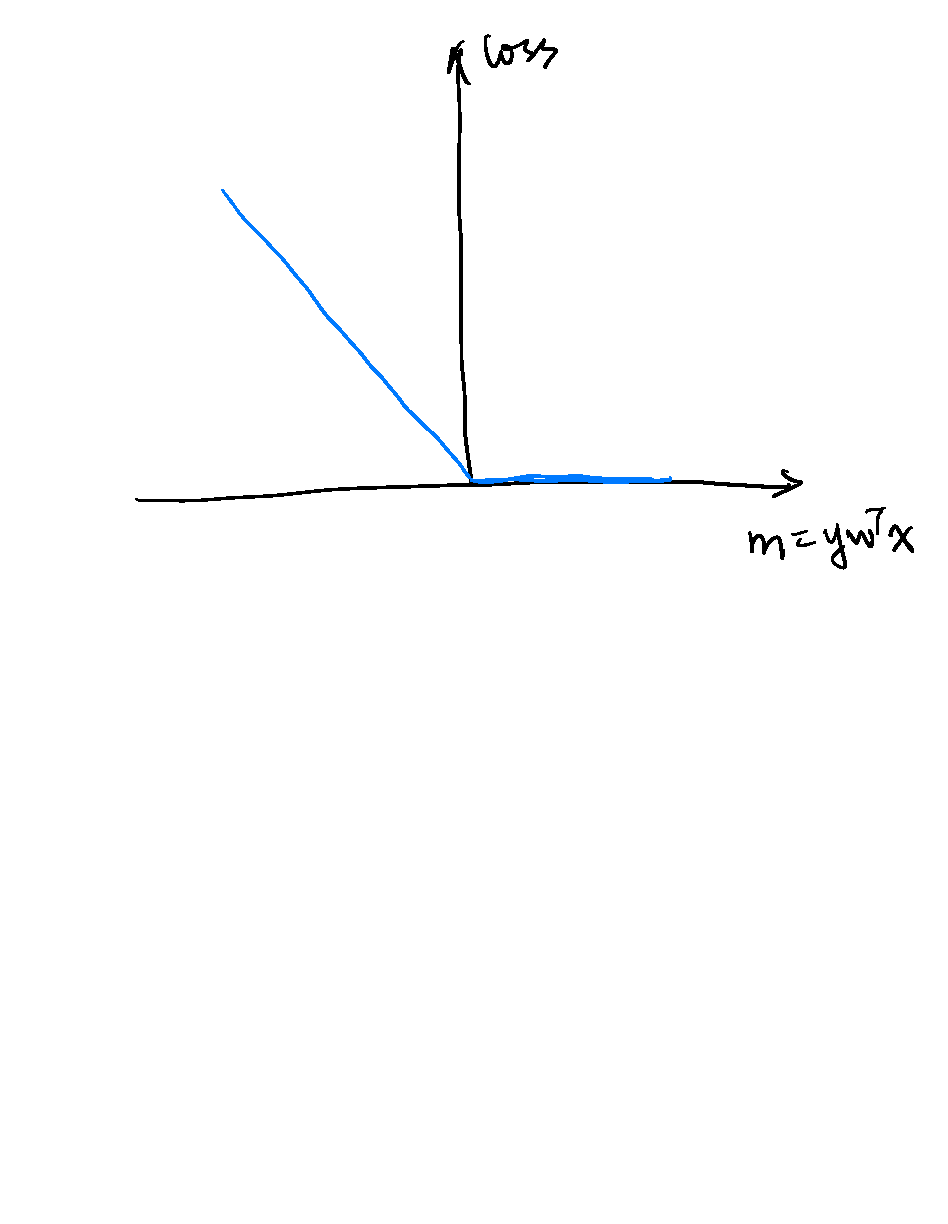
\includegraphics[height=0.5\textheight]{figures/perceptron-loss}
    \end{figure}
    If we do ERM with this loss function, what happens?
    %\pdfnote{
    %    Perceptron algorithm. Degenerate solution with w=0.
    %}
\end{frame}

\begin{frame}{Hinge Loss}
\begin{itemize}
\item SVM/Hinge loss: $\loss_{\text{Hinge}}=\max\left\{ 1-m,0\right\} =\left(1-m\right)_{+}$
\item Margin $m=yf(x)$; ``Positive part'' $(x)_{+}=x\ind{x\ge0}$.
\end{itemize}
\begin{center}
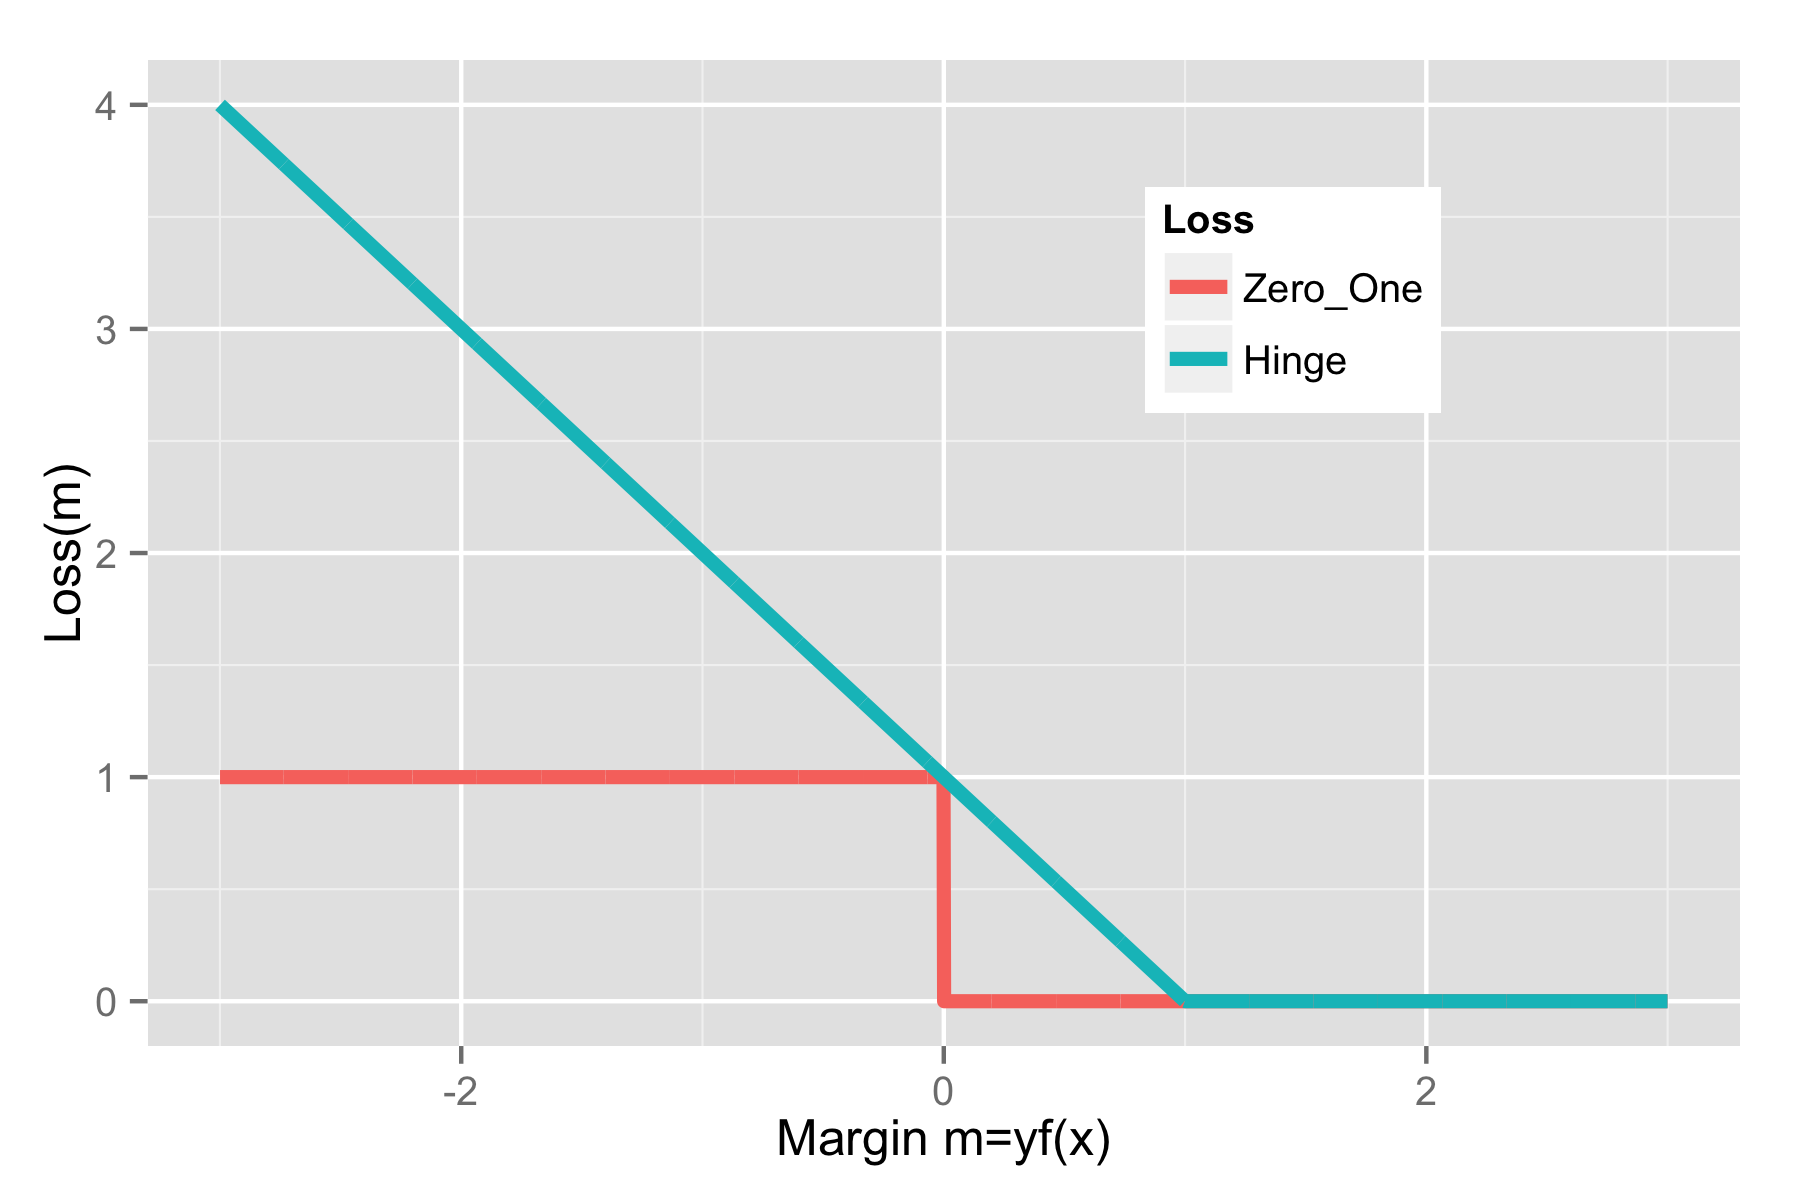
\includegraphics[height=0.5\textheight]{figures/loss.Zero_One.Hinge}
\par\end{center}

Hinge is a \textbf{convex}, \textbf{upper bound} on $0-1$ loss. Not
differentiable at $m=1$. \\
We have a \textbf{``margin error''} when $m<1$.
\end{frame}

\begin{frame}{Support Vector Machine}
    Using ERM:
\begin{itemize}
\item Hypothesis space $\cf=\left\{ f(x)=w^{T}x+b\mid w\in\reals^{d},b\in\reals\right\} $.
\item $\ell_{2}$ regularization (Tikhonov style)
\item Hinge loss $\ell(m)=\max\left\{ 1-m,0\right\} =\left(1-m\right)_{+}$
\item The SVM prediction function is the solution to
\[
\min_{w\in\reals^{d},b\in\reals}\frac{1}{2}||w||^{2}+\frac{c}{n}\sum_{i=1}^{n}\max\left(0,1-y_{i}\left[w^{T}x_{i}+b\right]\right).
\]
\item \al{Not differentiable} because of the $\max$
\end{itemize}
\end{frame}

\begin{frame}{SVM as a Constrained Optimization Problem}
\begin{itemize}
\item The SVM optimization problem is equivalent to
\begin{eqnarray*}
    \textrm{minimize} &  & \frac{1}{2}||w||^{2}+\frac{c}{n}\sum_{i=1}^{n}\xi_{i}\\
\textrm{subject to} &  & \xi_{i}\ge\max\left(0,1-y_{i}\left[w^{T}x_{i}+b\right]\right) \;\mbox{for }i=1,\ldots,n.
\end{eqnarray*}


\item Which is equivalent to
\begin{eqnarray*}
    \textrm{minimize} &  & \frac{1}{2}||w||^{2}+\frac{c}{n}\sum_{i=1}^{n}\xi_{i}\\
\textrm{subject to} &  & \xi_{i}\ge\left(1-y_{i}\left[w^{T}x_{i}+b\right]\right)\;\mbox{for }i=1,\ldots,n\\
 &  & \xi_{i}\ge0\;\mbox{for }i=1,\ldots,n
\end{eqnarray*}
\end{itemize}
\end{frame}

\begin{frame}
    {Summary}
    Two ways to derive the SVM optimization problem:
    \begin{itemize}
    \item Maximize the (geometric) margin
    \item Minimize the hinge loss with $\ell_2$ regularization
    \end{itemize}
    Both leads to the minimum norm solution satisfying certain margin constraints.

    \begin{itemize}
        \item \textbf{Hard-margin SVM}: all points must be correctly classified with the margin constraints
        \item \textbf{Soft-margin SVM}: allow for margin constraint violation with some penalty
    \end{itemize}
\end{frame}

\begin{frame}{Part II: Subgradient Descent for SVM}
    Now that we have the objective, can we do SGD on it?

    Subgradient: generalize gradient for non-differentiable convex functions
\end{frame}

\begin{frame}{SVM Optimization Problem (no intercept)}
\begin{itemize}
\item SVM objective function:
\[
    J(w)=\frac{1}{n}\sum_{i=1}^{n}\max\left(0,1-{y_{i}w^{T}x_{i}}\right)+\lambda||w||^{2}.
\]

\item Not differentiable... but let's think about gradient descent anyway.
\item Hinge loss: $\ell(m)=\max(0,1-m)$
%\item Derivative of hinge loss $\ell(m)=\max(0,1-m)$:
%\[
%\ell'(m)=\begin{cases}
%0 & m>1\\
%-1 & m<1\\
%\text{undefined} & m=1
%\end{cases}
%\]
\end{itemize}
\begin{eqnarray*}
\del_{w}J(w) & = & \del_{w}\left(\frac{1}{n}\sum_{i=1}^{n}\ell\left(y_{i}w^{T}x_{i}\right)+\lambda||w||^{2}\right)\\
 & = & \frac{1}{n}\sum_{i=1}^{n}\del_{w}\ell\left(y_{i}w^{T}x_{i}\right)+2\lambda w\\
% & = & \begin{cases}
%\frac{1}{n}\sum_{i:y_{i}w^{T}x_{i}<1}\left(-y_{i}x_{i}\right)+2\lambda w & \text{all }y_{i}w^{T}x_{i}\neq1\\
%\text{undefined} & \text{otherwise}
%\end{cases}
\end{eqnarray*}
\end{frame}

\begin{frame}{``Gradient'' of SVM Objective}
    \begin{itemize}
\item Derivative of hinge loss $\ell(m)=\max(0,1-m)$:
$$
\ell'(m)=\begin{cases}
0 & m>1\\
-1 & m<1\\
\text{undefined} & m=1
\end{cases}
$$

\item By chain rule, we have 
\begin{eqnarray*}
\del_{w}\ell\left(y_{i}w^{T}x_{i}\right) & = & \ell'\left(y_{i}w^{T}x_{i}\right)y_{i}x_{i}\\
& = & \begin{cases}
0 & y_{i}w^{T}x_{i}>1\\
-y_{i}x_{i} & y_{i}w^{T}x_{i}<1\\
\text{undefined} & y_{i}w^{T}x_{i}=1
\end{cases}
\end{eqnarray*}
\end{itemize}
\end{frame}

\begin{frame}{``Gradient'' of SVM Objective}

\begin{eqnarray*}
\del_{w}\ell\left(y_{i}w^{T}x_{i}\right) & = & \begin{cases}
0 & y_{i}w^{T}x_{i}>1\\
-y_{i}x_{i} & y_{i}w^{T}x_{i}<1\\
\text{undefined} & y_{i}w^{T}x_{i}=1
\end{cases}
\end{eqnarray*}

So 
    \vspace{-2ex}
\begin{eqnarray*}
\del_{w}J(w) & = & \del_{w}\left(\frac{1}{n}\sum_{i=1}^{n}\ell\left(y_{i}w^{T}x_{i}\right)+\lambda||w||^{2}\right)\\
 & = & \frac{1}{n}\sum_{i=1}^{n}\del_{w}\ell\left(y_{i}w^{T}x_{i}\right)+2\lambda w\\
 & = & \begin{cases}
\frac{1}{n}\sum_{i:y_{i}w^{T}x_{i}<1}\left(-y_{i}x_{i}\right)+2\lambda w & \text{all }y_{i}w^{T}x_{i}\neq1\\
\text{undefined} & \text{otherwise}
\end{cases}
\end{eqnarray*}
\end{frame}

\begin{frame}{Gradient Descent on SVM Objective?}
\begin{itemize}
\item The gradient of the SVM objective is
\[
\del_{w}J(w)=\frac{1}{n}\sum_{i:y_{i}w^{T}x_{i}<1}\left(-y_{i}x_{i}\right)+2\lambda w
\]
 when $y_{i}w^{T}x_{i}\neq1$ for all $i$, and \hl{otherwise
is undefined}.
\end{itemize}

Potential arguments for why we shouldn't care about the points of
nondifferentiability:\\
\begin{itemize}
\item If we start with a random $w$, will we ever hit exactly $y_{i}w^{T}x_{i}=1$?

\item If we did, could we perturb the step size by $\eps$ to miss such
a point?

\item Does it even make sense to check $y_{i}w^{T}x_{i}=1$ with floating
point numbers?
\end{itemize}
However, would gradient descent work if the objective is not differentiable?
\end{frame}

\section{Subgradient}
\begin{frame}{First-Order Condition for Convex, Differentiable Function}

\begin{itemize}
\item Suppose $f:\reals^{d}\to\reals$ is \hl{convex} and \hl{differentiable}
Then for any $x,y\in\reals^{d}$
\[
f(y)\ge f(x)+\del f(x)^{T}(y-x)
\]


\item The linear approximation to $f$ at $x$ is a \hl{global underestimator
}of $f$:
\begin{center}
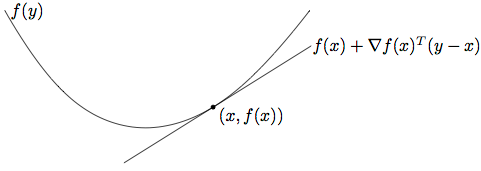
\includegraphics[width=0.5\columnwidth]{figures/BVFig3.2-convexTangent}
\par\end{center}
\item This implies that 
if $\del f(x)=0$ then $x$ is a global minimizer of $f$.
\end{itemize}
\let\thefootnote\relax\footnotetext{\tiny{Figure from Boyd \& Vandenberghe Fig. 3.2; Proof in Section 3.1.3 }}
\end{frame}

\begin{frame}{Subgradients}
\begin{definition}
    A vector $g\in\reals^{d}$ is a \textbf{subgradient} of a \emph{convex} function $f:\reals^{d}\to\reals$
at $x$ if for all $z$, 
$$
f(z)\ge f(x)+g^{T}(z-x).
$$
\end{definition}

\begin{center}
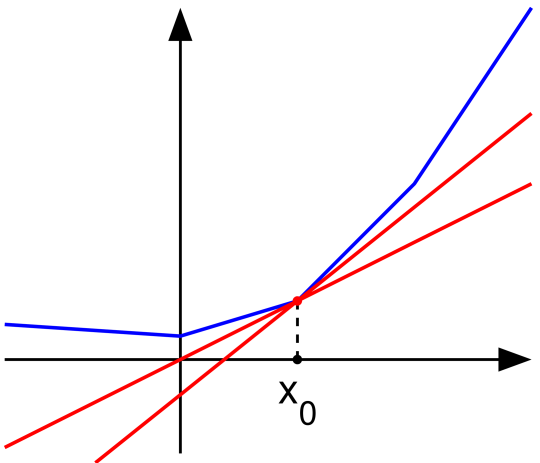
\includegraphics[height=0.4\textheight]{figures/Subderivative_illustration}
\par\end{center}

Blue is a graph of $f(x)$. \\
Each red line $x\mapsto f(x_{0})+g^{T}\left(x-x_{0}\right)$ is a
    \hl{global lower bound} on $f(x)$.
\end{frame}

\begin{frame}
    {Properties}
\begin{definitions}
\begin{itemize}
\item The set of all subgradients at $x$ is called the \textbf{subdifferential}:
$\partial f(x)$ 
\item $f$ is \textbf{subdifferentiable} at $x$ if $\exists$ at least
one subgradient at $x$. 
\end{itemize}
\end{definitions}

For convex functions:\\
    \begin{itemize}
        \setlength\itemsep{1ex}
\item $f$ is differentiable at $x$ iff $\partial f(x)=\left\{ \del f(x)\right\}$.
\item Subdifferential is always non-empty ($\partial f(x)=\emptyset \implies f$ is not convex)
\item $x$ is the global optimum iff $0\in\partial f(x)$.
    \end{itemize}

    For non-convex functions:\\
    \begin{itemize}
        \item The subdifferential may be an empty set (no global underestimator).
    \end{itemize}
\end{frame}

\begin{frame}{Subdifferential of Absolute Value}
\begin{itemize}
\item Consider $f(x)=\left|x\right|$

\end{itemize}
\let\thefootnote\relax\footnotetext{\tiny{Boyd EE364b: Subgradients Slides}}

\begin{center}
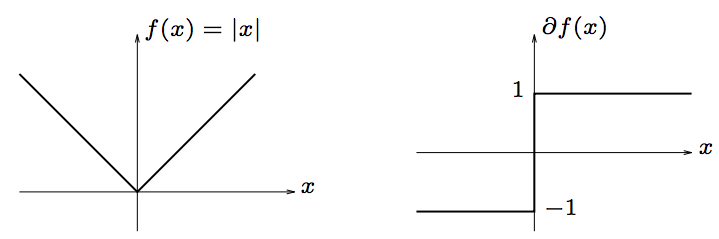
\includegraphics[width=0.8\columnwidth]{figures/subgradient-absolute-value}
\par\end{center}
\begin{itemize}
\item Plot on right shows $\left\{ (x,g)\mid x\in\reals,\;g\in\partial f(x)\right\} $ 
\end{itemize}
\end{frame}


\begin{frame}{Subgradients of $f(x_{1},x_{2})=\left|x_{1}\right|+2\left|x_{2}\right|$}
    \begin{columns}

        \begin{column}{0.6\textwidth}
\begin{itemize}
\item Let's find the subdifferential of $f(x_{1},x_{2})=\left|x_{1}\right|+2\left|x_{2}\right|$
at $\left(3,0\right)$.
\end{itemize}

\begin{itemize}
\item First coordinate of subgradient must be $1$, from $\left|x_{1}\right|$
part (at $x_{1}=3$).
\end{itemize}

\begin{itemize}
\item Second coordinate of subgradient can be anything in $\left[-2,2\right]$.
\end{itemize}

\begin{itemize}
\item So graph of $h(x_{1},x_{2})=f(3,0)+g^{T}\left(x_{1}-3,x_{2}-0\right)$
is a global underestimate of $f(x_{1},x_{2})$, for any $g=\left(g_{1},g_{2}\right),$
where $g_{1}=1$ and $g_{2}\in[-2,2]$. 
\end{itemize}
    \end{column}
        \begin{column}{0.3\textwidth}
\begin{center}
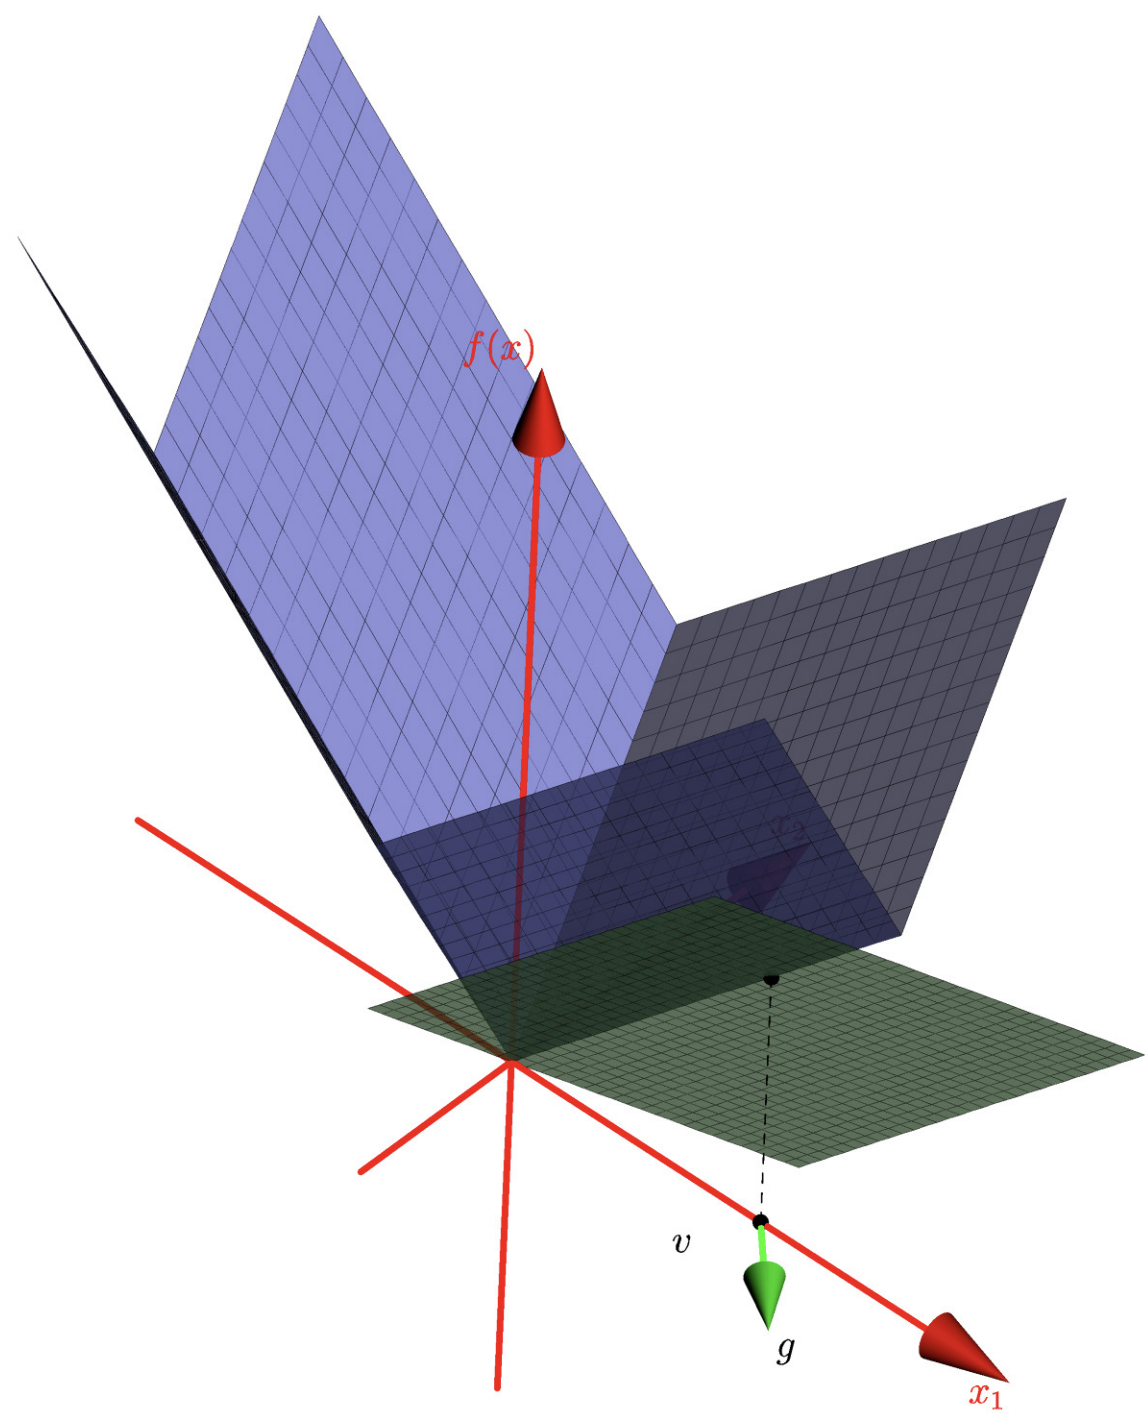
\includegraphics[height=0.75\textheight]{figures/underestimating-3d-plot-abs-x1-plus-2absx2}\let\thefootnote\relax\footnotetext{\tiny{Plot courtesy of Brett Bernstein.}} 
\par\end{center}
        \end{column}
    \end{columns}
\end{frame}

\begin{frame}{Subdifferential on Contour Plot}
\begin{center}
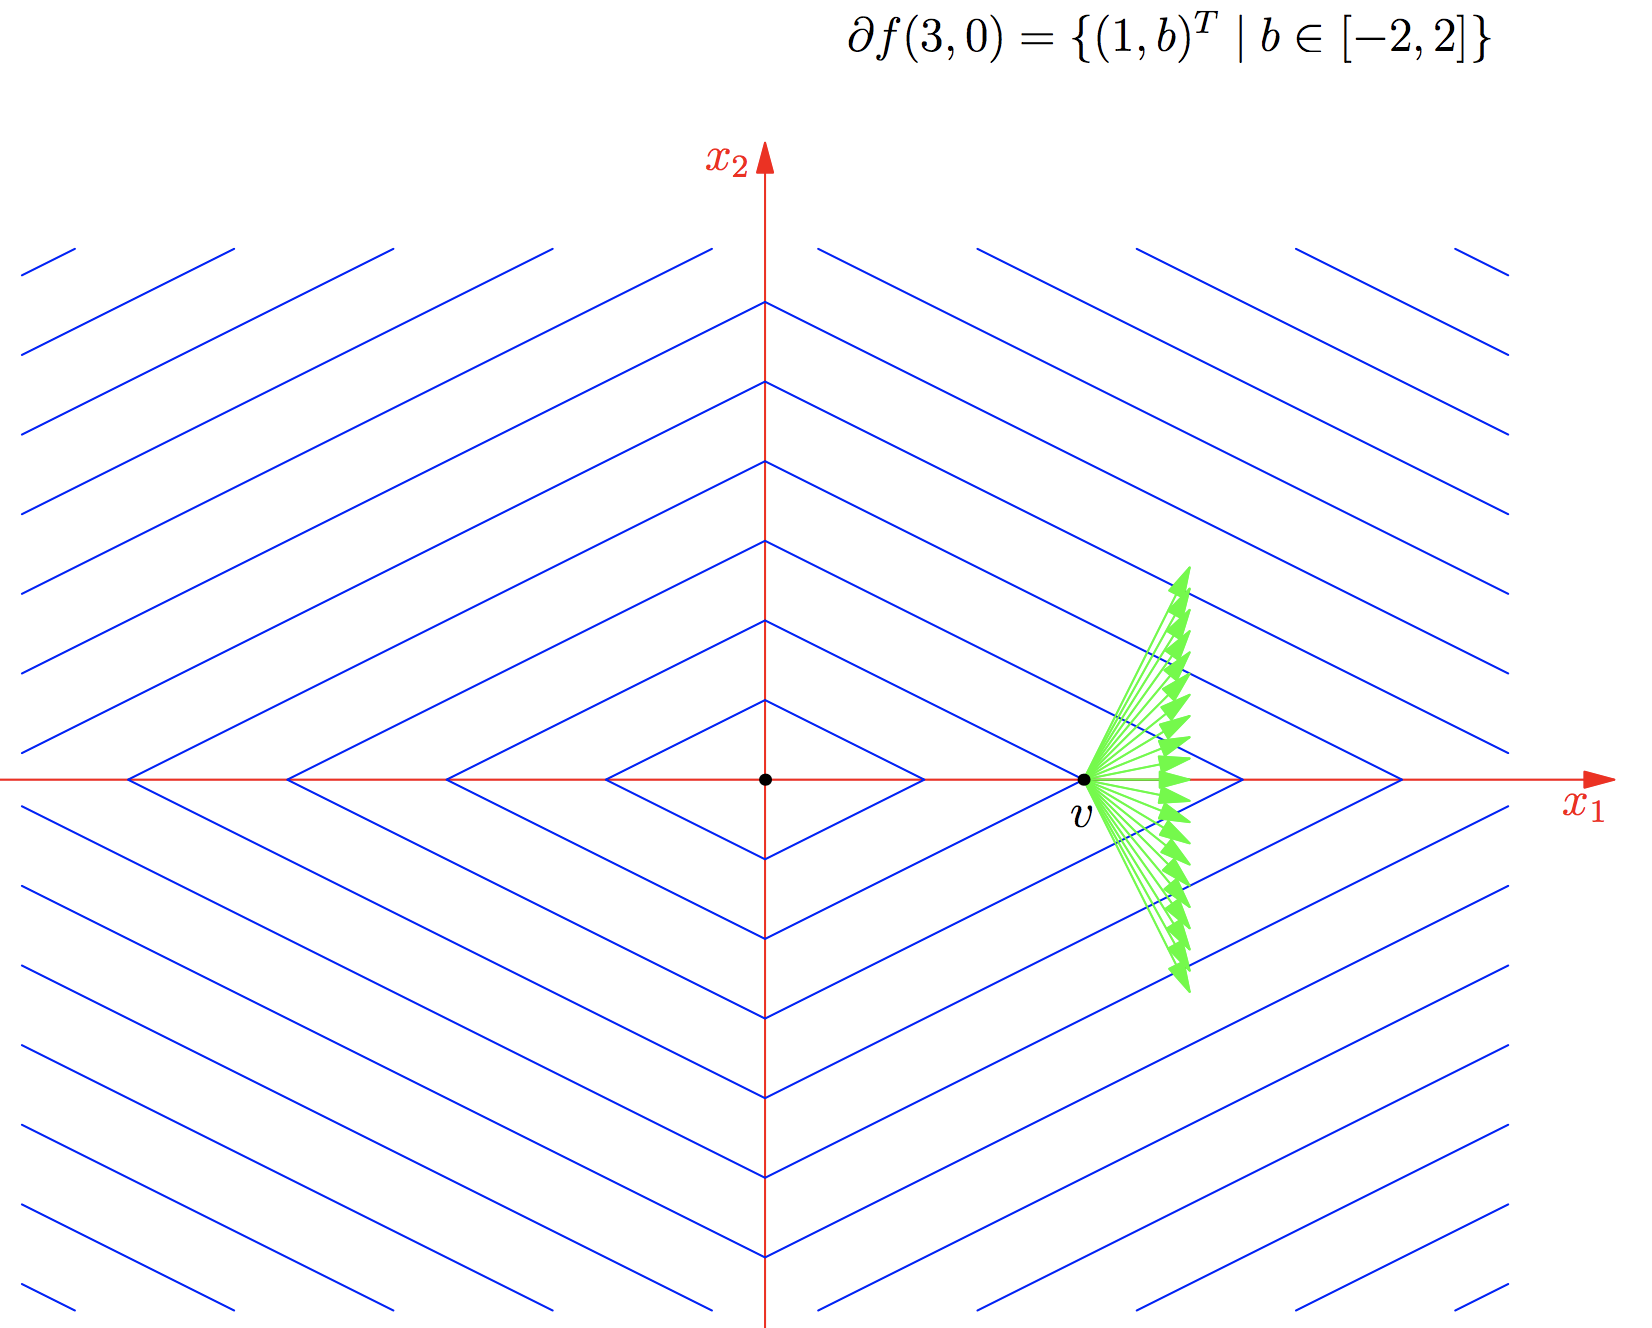
\includegraphics[height=0.6\textheight]{figures/subdiff-contour-plot-abs-x1-plus-2absx2}
\par\end{center}

\begin{center}
Contour plot of $f(x_{1},x_{2})=\left|x_{1}\right|+2\left|x_{2}\right|$,
with set of subgradients at $(3,0)$. .\let\thefootnote\relax\footnotetext{\tiny{Plot courtesy of Brett Bernstein.}}
\par\end{center}
\end{frame}

\begin{frame}
    {Basic Rules for Calculating Subdifferential}
    \begin{itemize}
        \item \head{Non-negative scaling}: $\partial \alpha f(x) = \alpha\partial f(x)$ for $(\alpha > 0)$
        \item \head{Summation}: $\partial(f_1(x) + f_2(x)) = d_1 + d_2$ for any $d_1\in\partial f_1$ and $d_2 \in\partial f_2$
        \item \head{Composing with affine functions}: $\partial f(Ax+b) = A^T\partial f(z)$ where $z=Ax+b$
        \item \head{max}: convex combinations of argmax gradients
            $$
            \partial \max(f_1(x), f_2(x)) =
            \begin{cases}
                \nabla f_1(x) & \text{if } f_1(x) > f_2(x), \\
                \nabla f_2(x) & \text{if } f_1(x) < f_2(x), \\
                \nabla \theta f_1(x) + (1-\theta)f_2(x) & \text{if } f_1(x) = f_2(x), \\
            \end{cases}
            $$
            where $\theta \in[0,1]$.
    \end{itemize}
\end{frame}

\section{Subgradient Descent}
\begin{frame}{Gradient orthogonal to level sets}
    We know that gradient points to the fastest ascent direction.
    What about subgradients?
\begin{center}
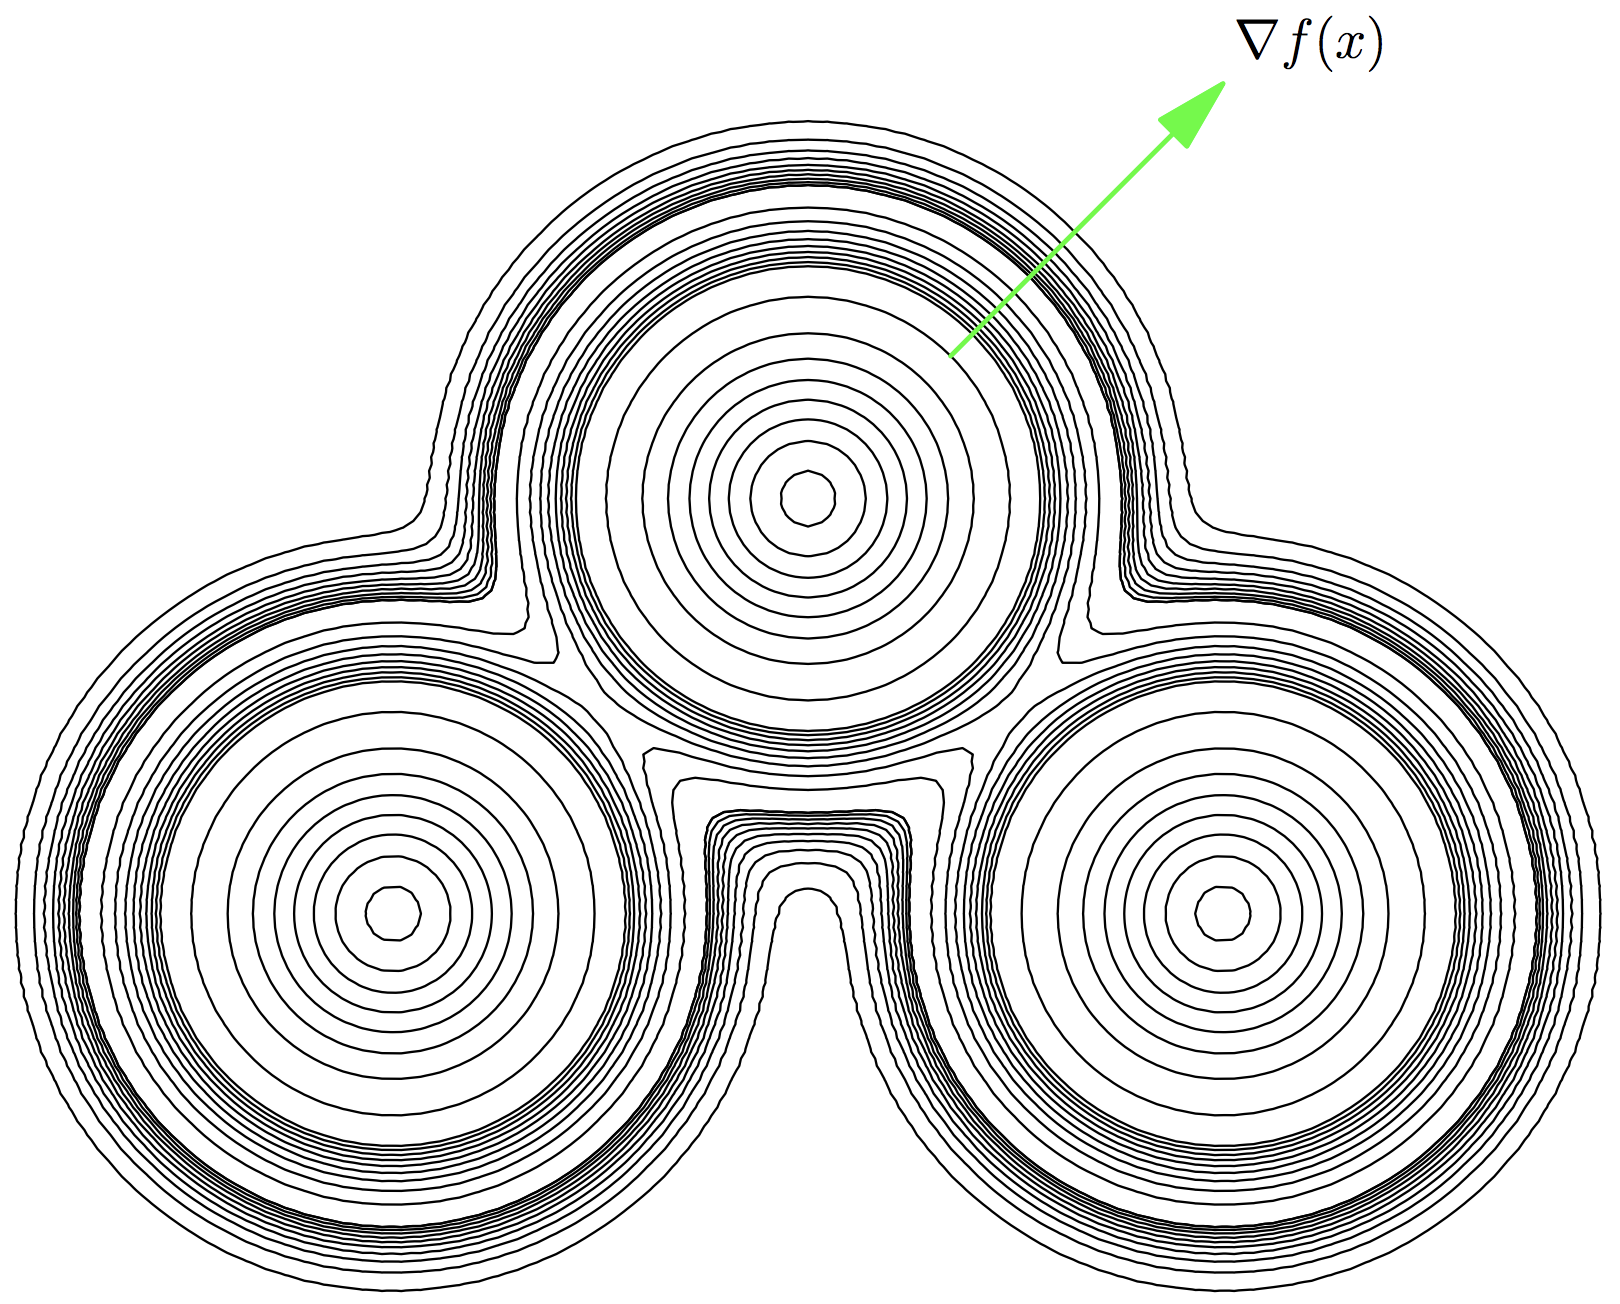
\includegraphics[height=0.6\textheight]{figures/grad-orthog-to-sublevel-sets}\let\thefootnote\relax\footnotetext{\tiny{Plot courtesy of Brett Bernstein.}}
\par\end{center}
\end{frame}

\begin{frame}{Contour Lines and Subgradients }
A hyperplane $H$ \textbf{supports} a set $S$ if $H$ intersects
$S$ and all of $S$ lies one one side of $H$.

    \head{Claim}: If $f:\reals^{d}\to\reals$ has subgradient $g$ at $x_{0}$, then
the hyperplane $H$ orthogonal to $g$ at $x_{0}$ must \textbf{support}
the level set $S=\left\{ x\in\reals^{d}\mid f(x)=f(x_{0})\right\} $. 

Proof:\\
\begin{itemize}
    \setlength\itemsep{1ex}
\item For any $y$, we have $f(y)\ge f(x_{0})+g^{T}(y-x_{0})$. (def
of subgradient)
\item If $y$ is strictly on side of $H$ that $g$ points in,
    \begin{itemize}
\item then $g^{T}\left(y-x_{0}\right)>0$.
\item So $f(y)>f(x_{0})$.
\item So $y$ is not in the level set $S$.
\end{itemize}
\item $\therefore$ All elements of $S$ must be on $H$ or on the $-g$
side of $H$.
\end{itemize}
\end{frame}

\begin{frame}{Subgradient of $f(x_{1},x_{2})=\left|x_{1}\right|+2\left|x_{2}\right|$ }
\begin{center}
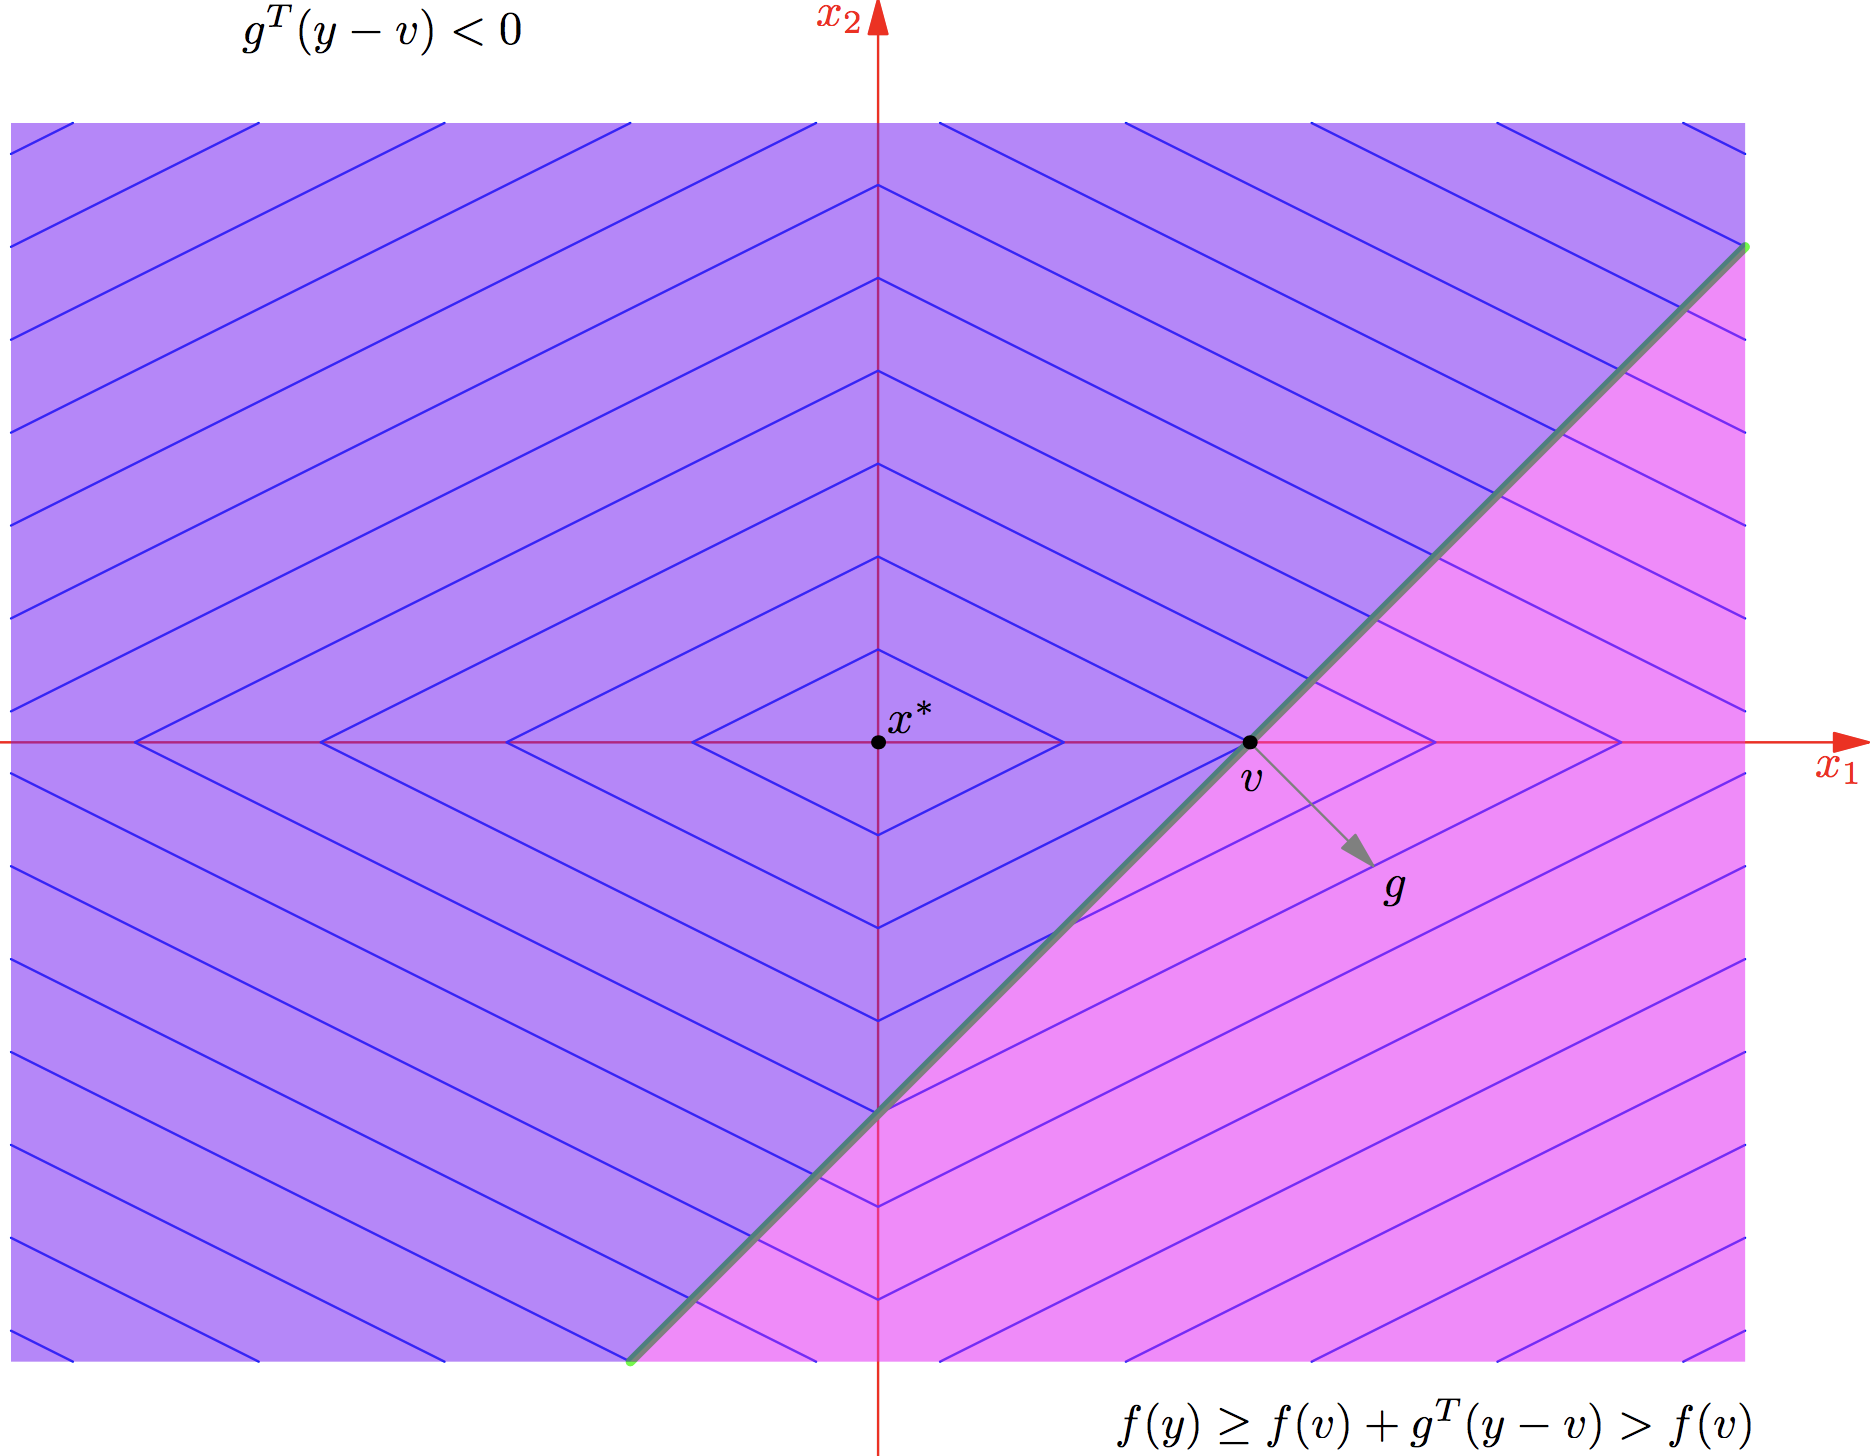
\includegraphics[height=0.6\textheight]{figures/contour-plot-abs-x1-plus-2absx2}\let\thefootnote\relax\footnotetext{\tiny{Plot courtesy of Brett Bernstein.}}
\par\end{center}
    \vspace{-1em}
\begin{itemize}
    \setlength\itemsep{1ex}
\item Points on $g$ side of $H$ have larger $f$-values than $f(x_{0})$.
(from proof)
\item But points on $-g$ side may \textbf{not }have smaller $f$-values. 
\item So $-g$ may \textbf{not} be a descent direction. (shown in figure)
\end{itemize}
\end{frame}

\begin{frame}
    {Subgradient Descent}
    \begin{itemize}
        \item Move along the negative subgradient:
            $$
            x^{t+1} = x^t - \eta g \quad \text{where } g\in\partial f(x^t) \text{ and } \eta > 0
            $$
        \item This can \al{increase} the objective but gets us \hl{closer to the minimizer} if $f$ is convex and $\eta$ is small enough:
            $$
            \|x^{t+1} - x^*\| < \|x^{t} - x^*\|
            $$
        \item Subgradients don't necessarily converge to zero as we get closer to $x^*$, so we need \al{decreasing step sizes}, e.g. $O(1/t)$ or $O(1/\sqrt{t})$.
        \item Subgradient methods are \al{slower} than gradient descent,
            e.g. ${\color{red}O(1/\epsilon^2)}$ vs $O(1/\epsilon)$ for convex functions.
    \end{itemize}
    \let\thefootnote\relax\footnotetext{\tiny{Based on \url{https://www.cs.ubc.ca/~schmidtm/Courses/5XX-S20/S4.pdf}}}
\end{frame}

\begin{frame}
    {Subgradient descent for SVM (HW3)}
SVM objective function:
    \vspace{-1em}
\[
    J(w)=\frac{1}{n}\sum_{i=1}^{n}\max\left(0,1-{y_{i}w^{T}x_{i}}\right)+\lambda||w||^{2}.
\]

    Pegasos: stochastic subgradient descent with step size $\eta_t = 1/(t\lambda)$
    \vspace{-1em}
    \begin{figure}
        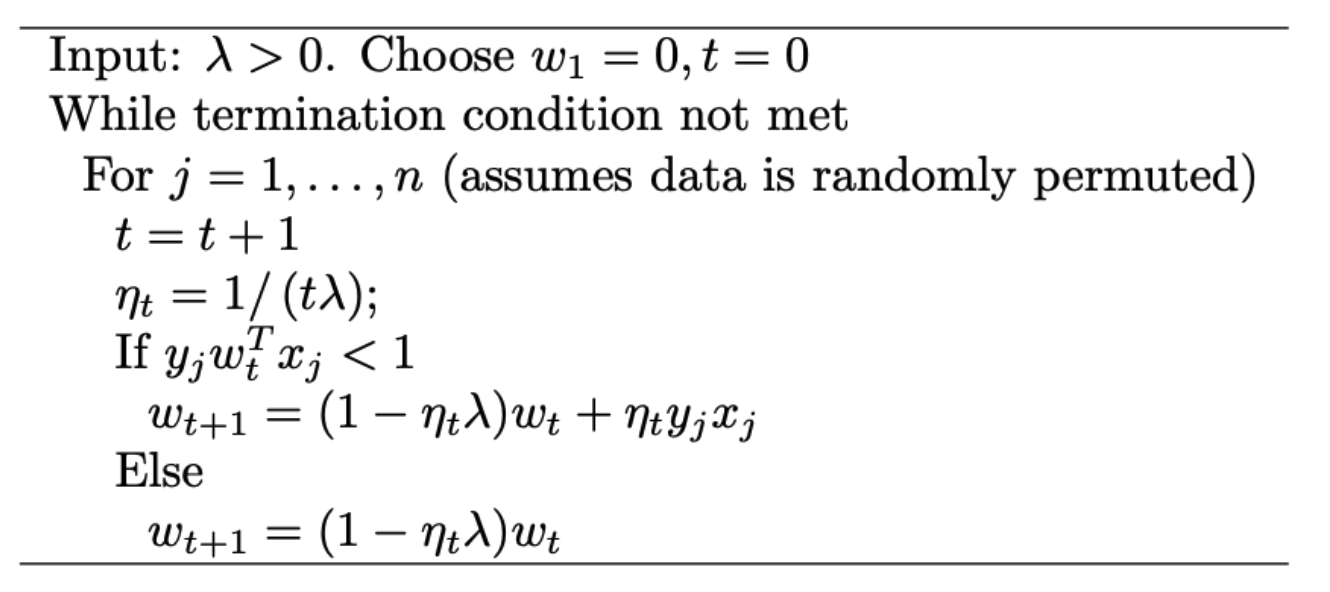
\includegraphics[height=0.5\textheight]{figures/pegasos}
    \end{figure}
\end{frame}

\begin{frame}
    {Summary}
    \begin{itemize}
        \item Subgradient: generalize gradient for non-differentiable convex functions
        \item Subgradient ``descent'':
            \begin{itemize}
                \item General method for non-smooth functions
                \item Simple to implement
                \item Slow to converge
            \end{itemize}
    \end{itemize}
\end{frame}

\begin{frame}{Part III: The Dual Problem}
    In addition to subgradient descent, we can directly solve the optimization problem using a QP solver.

    Let's study its dual problem to gain addition insights (which will be useful for next week!)
\end{frame}

\begin{frame}{SVM as a Quadratic Program}
\begin{itemize}
\item The SVM optimization problem is equivalent to
\begin{eqnarray*}
    \textrm{minimize} &  & \frac{1}{2}||w||^{2}+\frac{c}{n}\sum_{i=1}^{n}\xi_{i}\\
\textrm{subject to} &  & -\xi_{i}\le0\quad\mbox{for }i=1,\ldots,n\\
 &  & \left(1-y_{i}\left[w^{T}x_{i}+b\right]\right)-\xi_{i}\le0\quad\mbox{for }i=1,\ldots,n
\end{eqnarray*}

\item Differentiable objective function
\item $n+d+1$ unknowns and $2n$ affine constraints.
\item A \textbf{quadratic program} that can be solved by any off-the-shelf QP solver. 
\item Let's learn more by examining the dual.
\end{itemize}
\end{frame}

\section{Why Do We Care About the Dual?}

\begin{frame}{The Lagrangian}

The general {[}inequality-constrained{]} optimization problem is:
\begin{eqnarray*}
\textrm{minimize} &  & f_{0}(x)\\
\textrm{subject to} &  & f_{i}(x)\le0,\;\;i=1,\ldots,m
\end{eqnarray*}

\begin{definition}
The \textbf{Lagrangian} for this optimization problem is
\[
L(x,\lambda)=f_{0}(x)+\sum_{i=1}^{m}\lambda_{i}f_{i}(x).
\]
\end{definition}
\begin{itemize}
    \setlength\itemsep{1ex}
    \item $\lambda_{i}$'s are called \textbf{Lagrange multipliers} (also called the \textbf{dual variables}). 
    \item Weighted sum of the objective and constraint functions
    \item Hard constraints $\rightarrow$ soft constraints
\end{itemize}
\end{frame}

\begin{frame}
    {Lagrange Dual Function}
    \begin{definition}
        The \textbf{Lagrange dual function} is
        $$
        g(\lambda) = \inf_x L(x, \lambda)
        = \inf_x \p{f_{0}(x)+\sum_{i=1}^{m}\lambda_{i}f_{i}(x)}
        $$
    \end{definition}
    \begin{itemize}
        \item $g(\lambda)$ is \hl{concave}
            \note[item]{$g$ is concave because it is the infimum of affine functions. Note that we are not assuming convexity of $f_0$.}
        \item \textbf{Lower bound property}: if $\lambda \succeq 0$, $g(\lambda) \le p^*$ where $p^*$ is the optimal value of the optimization problem.
            \note[item]{Note that the proof is straightforward: $\sum_i\lambda_i f_i(x)$ is always negative.}
        \item $g(\lambda)$ can be $-\infty$ (uninformative lower bound)
            \note[item]{For example when $L(x,\lambda)$ is affine is $x$.}
    \end{itemize}
    \note[item]{We can consider $g(\lambda)$ as a parametrized lower bound that depends on $\lambda$. 
    So we might want to find $\lambda$ that gives us the best lower bound, which motivates the dual problem.}
\end{frame}

\begin{frame}{The Primal and the Dual}
\begin{itemize}
\item For any \textbf{primal form }optimization problem,
\begin{eqnarray*}
\textrm{minimize} &  & f_{0}(x)\\
\textrm{subject to} &  & f_{i}(x)\le0,\;\;i=1,\ldots,m,
\end{eqnarray*}
there is a recipe for constructing a corresponding \textbf{Lagrangian
dual problem:}
\begin{eqnarray*}
\textrm{maximize} &  & g(\lambda)\\
\textrm{subject to} &  & \lambda_{i}\ge0,\;\;i=1,\ldots,m,
\end{eqnarray*}

\item The dual problem is always a convex optimization problem.
\item The dual variables often have interesting and relevant interpretations.
\item The dual variables provide certificates for optimality.
\end{itemize}
\end{frame}

\begin{frame}{Weak Duality}
We always have \textbf{weak duality: }$p^{*}\ge d^{*}$.

\begin{center}
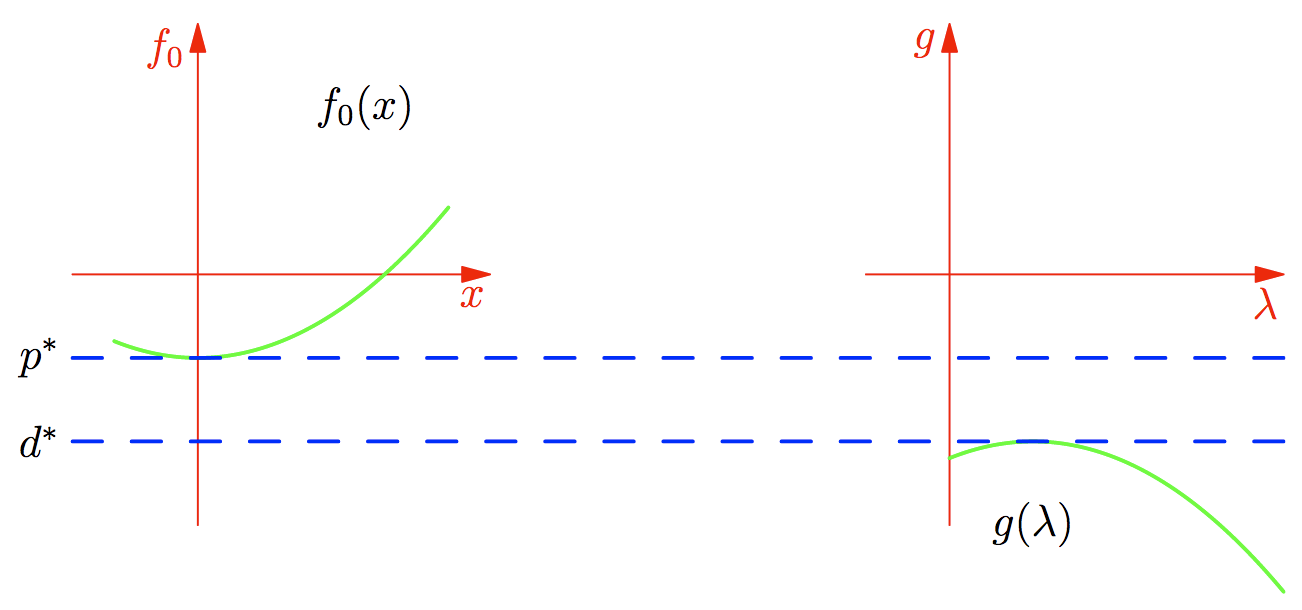
\includegraphics[height=0.6\textheight]{figures/weak-duality}
\par\end{center}

\let\thefootnote\relax\footnotetext{\tiny{Plot courtesy of Brett Bernstein.}}
\end{frame}

\begin{frame}{Strong Duality}

For some problems, we have \textbf{strong duality}: $p^{*}=d^{*}$.

\begin{center}
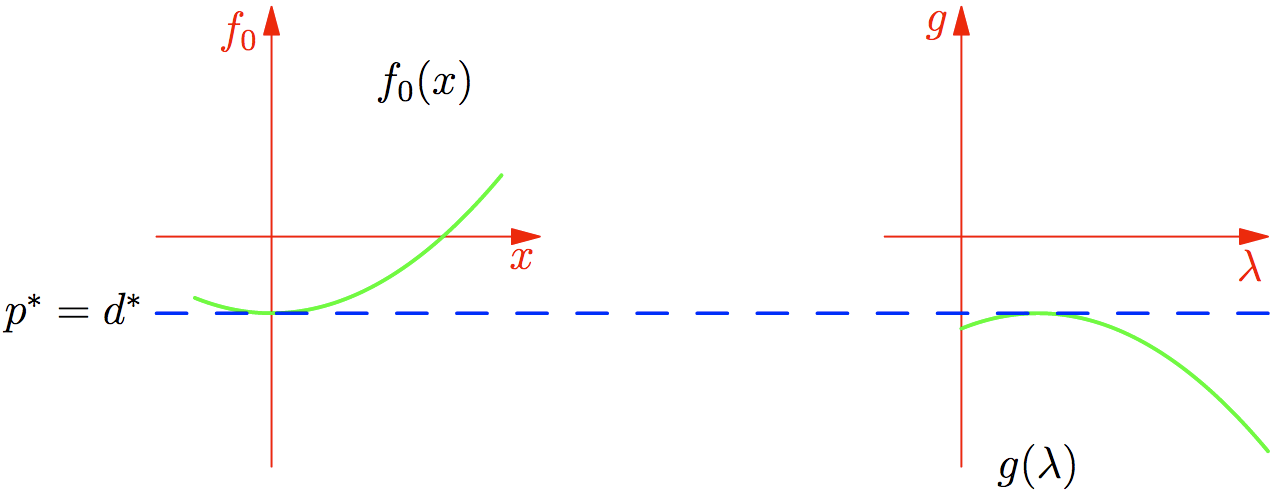
\includegraphics[height=0.6\textheight]{figures/strong-duality}
\par\end{center}

\vspace{-1em}
For convex problems, strong duality is fairly typical. 

\let\thefootnote\relax\footnotetext{\tiny{Plot courtesy of Brett Bernstein.}}
\end{frame}

\begin{frame}{Complementary Slackness}
\begin{itemize}
    \item \hl{Assume strong duality}. Let $x^{*}$ be primal optimal and $\lambda^{*}$ be dual optimal.
Then:
\begin{eqnarray*}
f_{0}(x^{*}) & = & g(\lambda^{*})=\inf_{x}\,L(x,\lambda^{*})\text{\quad(strong duality and definition)}\\
& \le & L(x^{*},\lambda^{*})\\
& = & f_{0}(x^{*})+\sum_{i=1}^{m}{\lambda_{i}^{*}f_{i}(x^{*})}\\
& \le & f_{0}(x^{*}).
\end{eqnarray*}

\end{itemize}
Each term in sum $\sum_{i=1}\lambda_{i}^{*}f_{i}(x^{*})$ must actually
be $0$. That is
\[
    \lambda_i > 0 \implies f_i(x^*) = 0 \quad\text{and}\quad
    f_i(x^*) < 0 \implies \lambda_i = 0 \quad \forall i
\]
This condition is known as \textbf{complementary slackness}. 
\end{frame}

\section{The SVM Dual Problem}
\begin{frame}{SVM Lagrange Multipliers}
    \vspace{-2em}
\begin{eqnarray*}
\textrm{minimize} &  & \frac{1}{2}||w||^{2}+\frac{c}{n}\sum_{i=1}^{n}\xi_{i}\\
\textrm{subject to} &  & -\xi_{i}\le0\quad\mbox{for }i=1,\ldots,n\\
 &  & \left(1-y_{i}\left[w^{T}x_{i}+b\right]\right)-\xi_{i}\le0\quad\mbox{for }i=1,\ldots,n
\end{eqnarray*}

\begin{center}
\begin{tabular}{|c|c|}
\hline 
Lagrange Multiplier & Constraint\tabularnewline
\hline 
\hline 
$\lambda_{i}$ & -$\xi_{i}\le0$\tabularnewline
\hline 
$\alpha_{i}$ & $\left(1-y_{i}\left[w^{T}x_{i}+b\right]\right)-\xi_{i}\le0$\tabularnewline
\hline 
\end{tabular}
\par\end{center}

\[
L(w,b,\xi,\alpha,\lambda)=\frac{1}{2}||w||^{2}+\frac{c}{n}\sum_{i=1}^{n}\xi_{i}+\sum_{i=1}^{n}\alpha_{i}\left(1-y_{i}\left[w^{T}x_{i}+b\right]-\xi_{i}\right)+\sum_{i=1}^{n}\lambda_{i}\left(-\xi_{i}\right)
\]

    \head{Dual optimum value}:
    $d^* = \sup_{\alpha,\lambda\succeq0}\inf_{w,b,\xi}L(w,b,\xi,\alpha,\lambda)$
    \note[item]{What are the primal and dual variables?}
\end{frame}

\begin{frame}
    {Strong Duality by Slater's Constraint Qualification}
The SVM optimization problem:
\begin{eqnarray*}
\textrm{minimize} &  & \frac{1}{2}||w||^{2}+\frac{c}{n}\sum_{i=1}^{n}\xi_{i}\\
\textrm{subject to} &  & -\xi_{i}\le0\;\mbox{for }i=1,\ldots,n\\
 &  & \left(1-y_{i}\left[w^{T}x_{i}+b\right]\right)-\xi_{i}\le0\;\mbox{for }i=1,\ldots,n
\end{eqnarray*}

Slater's constraint qualification:\\
    \begin{itemize}
\item Convex problem + affine constraints $\implies$strong duality iff
problem is feasible 
\item Do we have a feasible point?
    \note[item]{Constraints are satisfied by $w=b=0$ and $\xi_{i}=1$ for $i=1,\ldots,n$}
\item For SVM, we have \hl{strong duality}.
    \end{itemize}
\end{frame}

\begin{frame}{SVM Dual Function: First Order Conditions}

Lagrange dual function is the inf over primal variables of $L$: 
\begin{eqnarray*}
 &  & g(\alpha,\lambda)=\inf_{w,b,\xi}L(w,b,\xi,\alpha,\lambda)\\
 & = & \inf_{w,b,\xi}\left[\frac{1}{2}w^{T}w+\sum_{i=1}^{n}\xi_{i}\left(\frac{c}{n}-\alpha_{i}-\lambda_{i}\right)+\sum_{i=1}^{n}\alpha_{i}\left(1-y_{i}\left[w^{T}x_{i}+b\right]\right)\right]
\end{eqnarray*}
    \note[item]{How do we solve the minimization problem?}
    \note[item]{Is it convex? [yes, quadratic term]}

    \vspace{-2em}
\begin{eqnarray*}
\partial_{w}L=0 & \iff & w-\sum_{i=1}^{n}\alpha_{i}y_{i}x_{i}=0\;\iff\;\boxed{w=\sum_{i=1}^{n}\alpha_{i}y_{i}x_{i}}\\
\partial_{b}L=0 & \iff & -\sum_{i=1}^{n}\alpha_{i}y_{i}=0\;\iff\;\boxed{\sum_{i=1}^{n}\alpha_{i}y_{i}=0}\\
\partial_{\xi_{i}}L=0 & \iff & \frac{c}{n}-\alpha_{i}-\lambda_{i}=0\;\iff\;\boxed{\alpha_{i}+\lambda_{i}=\frac{c}{n}}
\end{eqnarray*}
\end{frame}

\begin{frame}{SVM Dual Function}
\begin{itemize}
    \setlength\itemsep{1ex}
\item Substituting these conditions back into $L$, the second term disappears.
\item First and third terms become 
\begin{eqnarray*}
\frac{1}{2}w^{T}w & = & \frac{1}{2}\sum_{i,j=1}^{n}\alpha_{i}\alpha_{j}y_{i}y_{j}x_{i}^{T}x_{j}\\
\sum_{i=1}^{n}\alpha_{i}(1-y_{i}\left[w^{T}x_{i}+b\right]) & = & \sum_{i=1}^{n}\alpha_{i}-\sum_{i,j=1}^{n}\alpha_{i}\alpha_{j}y_{i}y_{j}x_{j}^{T}x_{i}-b\underbrace{\sum_{i=1}^{n}\alpha_{i}y_{i}}_{=0}.
\end{eqnarray*}

        \vspace{-2ex}
\item Putting it together, the dual function is 
\[
g(\alpha,\lambda)=\begin{cases}
\sum_{i=1}^{n}\alpha_{i}-\frac{1}{2}\sum_{i,j=1}^{n}\alpha_{i}\alpha_{j}y_{i}y_{j}x_{j}^{T}x_{i} & \substack{\substack{\sum_{i=1}^{n}\alpha_{i}y_{i}=0\\
\alpha_{i}+\lambda_{i}=\frac{c}{n}\mbox{, all }i
}
}
\\
-\infty & \mbox{otherwise.}
\end{cases}
\]
\end{itemize}
\end{frame}

\begin{frame}{SVM Dual Problem}
\begin{itemize}
\item The \textbf{dual function} is
\[
g(\alpha,\lambda)=\begin{cases}
\sum_{i=1}^{n}\alpha_{i}-\frac{1}{2}\sum_{i,j=1}^{n}\alpha_{i}\alpha_{j}y_{i}y_{j}x_{j}^{T}x_{i} & \substack{\substack{\sum_{i=1}^{n}\alpha_{i}y_{i}=0\\
\alpha_{i}+\lambda_{i}=\frac{c}{n}\mbox{, all }i
}
}
\\
-\infty & \mbox{otherwise.}
\end{cases}
\]


\item The \textbf{dual problem }is $\sup_{\alpha,\lambda\succeq0}g(\alpha,\lambda)$:
\begin{eqnarray*}
\sup_{\alpha,\lambda} &  & \sum_{i=1}^{n}\alpha_{i}-\frac{1}{2}\sum_{i,j=1}^{n}\alpha_{i}\alpha_{j}y_{i}y_{j}x_{j}^{T}x_{i}\\
\mbox{s.t.} &  & \sum_{i=1}^{n}\alpha_{i}y_{i}=0\\
 & \quad & \alpha_{i}+\lambda_{i}=\frac{c}{n}\quad\alpha_{i},\lambda_{i}\ge0,\;i=1,\ldots,n
\end{eqnarray*}
 
\end{itemize}
\end{frame}

\section{Insights from the Dual Problem}
\begin{frame}
    {KKT Conditions}
    For \hl{convex} problems, if \hl{Slater's condition} is satisfied, then \textbf{KKT conditions} provide \hl{necessary and sufficient} conditions for the optimal solution.
    \begin{itemize}
        \item Primal feasibility: $f_i(x) \le 0 \quad \forall i$
        \item Dual feasibility: $\lambda \succeq 0$
        \item Complementary slackness: $\lambda_i f_i(x)=0$
        \item First-order condition:
            $$
            \frac{\partial}{\partial x} L(x, \lambda) = 0
            $$
            \note[item]{$x$ needs to be a stationary point of the Lagrangian.}
    \end{itemize}
\end{frame}

\begin{frame}{The SVM Dual Solution}
\begin{itemize}
\item We found the SVM dual problem can be written as:
\begin{eqnarray*}
\sup_{\alpha} &  & \sum_{i=1}^{n}\alpha_{i}-\frac{1}{2}\sum_{i,j=1}^{n}\alpha_{i}\alpha_{j}y_{i}y_{j}x_{j}^{T}x_{i}\\
\mbox{s.t.} &  & \sum_{i=1}^{n}\alpha_{i}y_{i}=0\\
 & \quad & \alpha_{i}\in\left[0,\frac{c}{n}\right]\;i=1,\ldots,n.
\end{eqnarray*}
\end{itemize}

\begin{itemize}
\item Given solution $\alpha^{*}$ to dual, primal solution is $w^{*}=\sum_{i=1}^{n}\alpha_{i}^{*}y_{i}x_{i}$. 
\item The solution is in the space spanned by the inputs.
\item Note $\alpha_{i}^{*}\in[0,\frac{c}{n}]$. So $c$ controls max weight
on each example. (\textbf{Robustness}!)
        \begin{itemize}
            \item What's the relation between $c$ and regularization?
                \note[item]{If $c$ is small, the solution is not sensitive to any single example---strong regularization. We can also see this in the primal problem: small $c$ corresponds to larger coefficients for the regularization term.}
        \end{itemize}
\end{itemize}
\end{frame}

\begin{frame}{Complementary Slackness Conditions}
\begin{itemize}
\item Recall our primal constraints and Lagrange multipliers:
\end{itemize}
\begin{center}
\begin{tabular}{|c|c|}
\hline 
Lagrange Multiplier & Constraint\tabularnewline
\hline 
\hline 
$\lambda_{i}$ & -$\xi_{i}\le0$\tabularnewline
\hline 
$\alpha_{i}$ & $\left(1-y_{i}f(x_{i})\right)-\xi_{i}\le0$\tabularnewline
\hline 
\end{tabular}
\par\end{center}

\begin{itemize}
\item Recall first order condition $\del_{\xi_{i}}L=0$ gave us $\lambda_{i}^{*}=\frac{c}{n}-\alpha_{i}^{*}$.
\item By strong duality, we must have \textbf{complementary slackness}:
\begin{align*}
\alpha_{i}^{*}\left(1-y_{i}f^{*}(x_{i})-\xi_{i}^{*}\right) & =0\\
\lambda_{i}^{*}\xi_{i}^{*}=\left(\frac{c}{n}-\alpha_{i}^{*}\right)\xi_{i}^{*} & =0
\end{align*}
\end{itemize}
\end{frame}

\begin{frame}{Consequences of Complementary Slackness}
By strong duality, we must have \textbf{complementary slackness}.
\begin{align*}
\alpha_{i}^{*}\left(1-y_{i}f^{*}(x_{i})-\xi_{i}^{*}\right) & =0\\
\left(\frac{c}{n}-\alpha_{i}^{*}\right)\xi_{i}^{*} & =0
\end{align*}

Recall ``\textbf{slack variable}'' $\xi_{i}^{*}=\max\left(0,1-y_{i}f^{*}(x_{i})\right)$
is the hinge loss on $\left(x_{i},y_{i}\right)$.
\begin{itemize}
\item If $y_{i}f^{*}(x_{i})>1$ then the margin loss is $\xi_{i}^{*}=0$,
and we get $\alpha_{i}^{*}=0$.
\item If $y_{i}f^{*}(x_{i})<1$ then the margin loss is $\xi_{i}^{*}>0$,
so $\alpha_{i}^{*}=\frac{c}{n}$. 

\item If $\alpha_{i}^{*}=0$, then $\xi_{i}^{*}=0$, which implies no loss,
so $y_{i}f^{*}(x)\ge1$.

\item If $\alpha_{i}^{*}\in\left(0,\frac{c}{n}\right)$, then $\xi_{i}^{*}=0$,
which implies $1-y_{i}f^{*}(x_{i})=0$.
\end{itemize}
\end{frame}

\begin{frame}{Complementary Slackness Results: Summary}
If $\alpha^{*}$ is a solution to the dual problem, then primal solution
is 
\[
w^{*}=\sum_{i=1}^{n}\alpha_{i}^{*}y_{i}x_{i}
    \quad \text{where} \alpha_{i}^{*}\in[0,\frac{c}{n}] .
\]

    Relation between margin and example weights ($\alpha_i$'s):
\begin{eqnarray*}
\alpha_{i}^{*}=0 & \implies & y_{i}f^{*}(x_{i})\ge1\\
\alpha_{i}^{*}\in\left(0,\frac{c}{n}\right) & \implies & y_{i}f^{*}(x_{i})=1\\
\alpha_{i}^{*}=\frac{c}{n} & \implies & y_{i}f^{*}(x_{i})\le1
\end{eqnarray*}
\begin{eqnarray*}
y_{i}f^{*}(x_{i})<1 & \implies & \alpha_{i}^{*}=\frac{c}{n}\\
y_{i}f^{*}(x_{i})=1 & \implies & \alpha_{i}^{*}\in\left[0,\frac{c}{n}\right]\\
y_{i}f^{*}(x_{i})>1 & \implies & \alpha_{i}^{*}=0
\end{eqnarray*}
\end{frame}

\begin{frame}{Support Vectors}
\begin{itemize}
\item If $\alpha^{*}$ is a solution to the dual problem, then primal solution
is 
\[
w^{*}=\sum_{i=1}^{n}\alpha_{i}^{*}y_{i}x_{i}
\]
with $\alpha_{i}^{*}\in[0,\frac{c}{n}]$. 

\item The $x_{i}$'s corresponding to $\alpha_{i}^{*}>0$ are called \textbf{support
vectors.}

\item Few margin errors or ``on the margin'' examples $\implies$ \hl{sparsity
in input examples}.
\end{itemize}
\end{frame}

%\begin{frame}{The Bias Term: $b$}
%\begin{itemize}
%\item For our SVM primal, the complementary slackness conditions are:
%\begin{align}
%\alpha_{i}^{*}\left(1-y_{i}\left[x_{i}^{T}w^{*}+b\right]-\xi_{i}^{*}\right) & =0\label{eq:lossNonNegativeSlackCondition-1}\\
%\lambda_{i}^{*}\xi_{i}^{*}=\left(\frac{c}{n}-\alpha_{i}^{*}\right)\xi_{i}^{*} & =0\label{eq:marginLossSlackCondition-1}
%\end{align}
%
%
%\item Suppose there's an $i$ such that $\alpha_{i}^{*}\in\left(0,\frac{c}{n}\right)$.
%
%\item \eqref{eq:marginLossSlackCondition-1} implies $\xi_{i}^{*}=0$.
%
%\item \eqref{eq:lossNonNegativeSlackCondition-1} implies 
%\begin{eqnarray*}
% &  & y_{i}\left[x_{i}^{T}w^{*}+b^{*}\right]=1\\
% & \iff & x_{i}^{T}w^{*}+b^{*}=y_{i}\mbox{ (use }y_{i}\in\left\{ -1,1\right\} )\\
% & \iff & \boxed{b^{*}=y_{i}-x_{i}^{T}w^{*}}
%\end{eqnarray*}
%\end{itemize}
%\end{frame}
%
%\begin{frame}{The Bias Term: $b$}
%\begin{itemize}
%\item We get the same $b^{*}$ for any choice of $i$ with $\alpha_{i}^{*}\in\left(0,\frac{c}{n}\right)$ 
%\[
%b^{*}=y_{i}-x_{i}^{T}w^{*}
%\]
%
%\item With numerical error, more robust to average over all eligible $i$'s:
%\[
%b^{*}=\text{mean}\left\{ y_{i}-x_{i}^{T}w^{*}\mid\alpha_{i}^{*}\in\left(0,\frac{c}{n}\right)\right\} .
%\]
%
%\item If there are no $\alpha_{i}^{*}\in\left(0,\frac{c}{n}\right)$?
%\begin{itemize}
%\item Then we have a \textbf{degenerate SVM training problem}\footnote{See Rifkin et al.'s ``A Note on Support Vector Machine Degeneracy'',
%an MIT AI Lab Technical Report.} ($w^{*}=0$).
%\end{itemize}
%\end{itemize}
%\end{frame}

\section{Teaser for Kernelization}

\begin{frame}{Dual Problem: Dependence on $x$ through inner products}
\begin{itemize}
\item SVM Dual Problem:
\begin{eqnarray*}
\sup_{\alpha} &  & \sum_{i=1}^{n}\alpha_{i}-\frac{1}{2}\sum_{i,j=1}^{n}\alpha_{i}\alpha_{j}y_{i}y_{j}x_{j}^{T}x_{i}\\
\mbox{s.t.} &  & \sum_{i=1}^{n}\alpha_{i}y_{i}=0\\
 & \quad & \alpha_{i}\in\left[0,\frac{c}{n}\right]\;i=1,\ldots,n.
\end{eqnarray*}


\item Note that all dependence on inputs $x_{i}$ and $x_{j}$ is through
their inner product: $\left\langle x_{j},x_{i}\right\rangle =x_{j}^{T}x_{i}$.

\item We can replace $x_{j}^{T}x_{i}$ by other products... 

\item This is a ``kernelized'' objective function. 
\end{itemize}
\end{frame}
\end{document}
